\documentclass{article}
\usepackage{geometry}
\newgeometry{vmargin={18mm}, hmargin={20mm,20mm}}
\usepackage[export]{adjustbox}[2011/08/13]
\usepackage{subcaption}
\usepackage{placeins}
\usepackage[backend=biber, giveninits=true]{biblatex}
\usepackage{graphicx}
\usepackage{color}
\usepackage{listings}
\lstset{basicstyle=\ttfamily}
\usepackage{caption}
\usepackage{amsmath}
\usepackage{amssymb}
\usepackage{amsthm}
\usepackage{siunitx} %This is currently a prealpha version that I got by accident
\usepackage{dcolumn}% Align table columns on decimal point
\usepackage{latexsym}
\usepackage{bm}
\usepackage{multirow}
\usepackage{cancel}
\usepackage{float}
\usepackage{booktabs}
\usepackage{rotating}

% make table
\definecolor{tableHeader}{gray}{0.5}
\definecolor{tableShade}{gray}{0.9}
\usepackage{tabularx}
\usepackage[table]{xcolor}
\newcolumntype{R}{>{\raggedright\arraybackslash}X}
\newcolumntype{C}{>{\centering\arraybackslash}X}

\let\vec\mathbf
\newcommand{\homejet}{\lstinline{Traditional}}
\newcommand{\fastjet}{\lstinline{FastJet}}
\newcommand{\spectralmeanjet}{\lstinline{SpectralMeanJet}}
\newcommand{\spectralfulljet}{\lstinline{SpectralFullJet}}
\newcommand{\splittingjet}{\lstinline{SplittingJet}}
\newcommand{\indicatorjet}{\lstinline{IndicatorJet}}
\newcommand{\stoppingdeltar}{\ensuremath{\Delta R}}
\newcommand{\distancedeltar}{\ensuremath{\Delta R'}}
\newcommand{\beau}{\ensuremath{b}}
\newcommand{\bbar}{\ensuremath{\bar{b}}}
\newcommand{\bthing}[1]{\ensuremath{b\text{-#1}}}
\def\AZH{\(A \rightarrow ZH\)}
\def\Hbb{\(H \rightarrow b\bar{b}\)}
\def\Abb{\(A \rightarrow b\bar{b}\)}
\def\HZA{\(H \rightarrow ZA\)}
\bibliography{writeup}
\graphicspath{{./graphics/}}
\begin{document}
\title{Machine learning on High Energy Physics}
\author{H.A. Day-Hall \\ {\small Supervisors; S. Dasmahpatra, S. Moretti, C.H. Shepherd-Themistocleous}}
	
	\maketitle
	
	\tableofcontents
    \FloatBarrier
    %\begin{abstract}
    %    Stuff
	%\end{abstract}
     
    \FloatBarrier
    \section{Introduction}

I am a student from the NGCM,
an interdisciplinary doctoral training centre focused on 
computational problem solving across STEM fields.
The investigations presented here straddle a number of topics, machine learning, high energy experimental physics and high energy phenomenology. 
This has been possible thanks to training
from both the physics and computer science departments
during the first year of this course,
and continued feedback at conferences and workshops, detailed in section~\ref{sec:presentations}.

Stefano Moretti (Physics, Univeristy of Southampton) provides supervision and guidance on the phenomenology aspect,
Claire Shepherd-Themistocleous (CMS, Rutherford Appleton Laboratory) provides supervision with experimental expertises and
Srinandan Dasmahapatra (Computer Science, University of Southampton) provides supervision with regards to machine learning.




    \FloatBarrier
    \section{Problem Statement and outline}
Particle colliders such as the LHC grant insight into physics by
creating heavy short lived particles that do not occur without a high energy collision
and only persist for a fraction of a second before decaying into lighter particles.
There is then a sequence of decays, known as a shower, before something
stable and long live enough to reach the detectors is created.
From the remnants of the decay that reach the detector we seek
to characterise the heavy particle created in the collision.

The data pipeline can be seen as a whole in~\cite{Stoye_DeepCMS2018, Schramm:2291608}.
Evidence of the shower is gathered from multiple concentric detectors about the collision point, the primary components being the 
silicon tracker for charged particles and the calorimeter for neutral particles. 
These can be seen in figure~\ref{fig:lit_CMSdetector}.
\begin{figure}
    \centering
    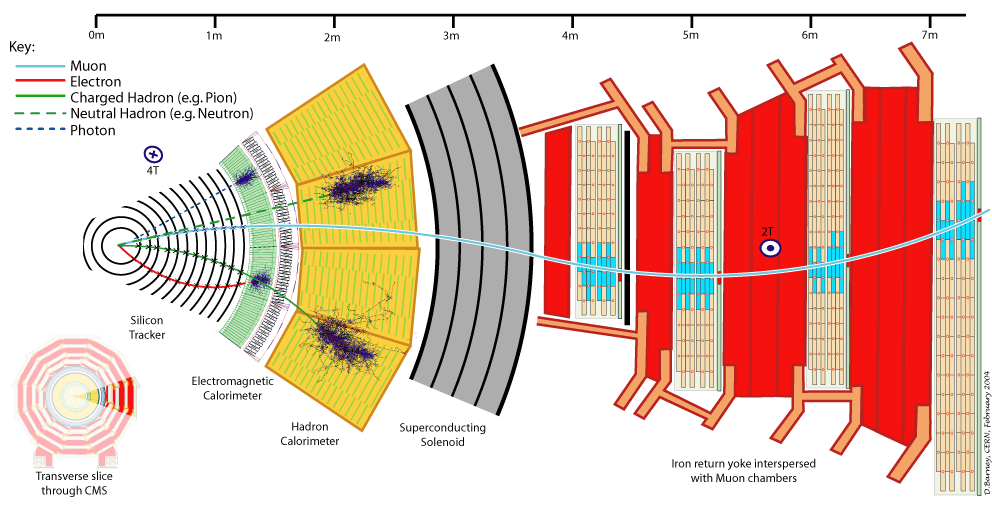
\includegraphics[width=0.8\textwidth]{images/lit_CMSdetector.png}
    \caption{The CMS detector has a concentric structure with each layer sensitive to a subset of possible particles.
             \cite{Stoye_DeepCMS2018}}
             % ADD could add more to this caption
    \label{fig:lit_CMSdetector}
\end{figure}
This data is essentially a series of energy deposits associated with three dimensional coordinates,
there is no time stamp available because the interaction occurs faster than the electronics can read out.
At this point the Particle Flow algorithm is used to reconstruct four vector tracks from the readings~\cite{Beaudette_particleFlow2013}.

%A signal of particular interest is found in the extended Higgs sector.
%Since the discovery of the Higgs Boson in 2012, it's couplings
%have been seen to be in agreement with the Standard Model (SM),
%however additional Higgs particles remain possible.
%The second doublet of the 2HDM allows a further 5 particles;
%two CP even (\(h\) and \(H\), with, conventionally, \(m_h < m_H\)),
%one CP odd (\(A\))
%and a pair of charged (\(H^\pm\)) Higgs bosons.
One possibility under investigation in these experiments is that of an extended Higgs sector
such as the two Higgs Doublet model (2HDM)~\cite{Branco2012THDM}.
The 2HDM introduces 5 new particles;
two CP even (\(h\) and \(H\), with, conventionally, \(m_h < m_H\)),
one CP odd (\(A\))
and a pair of charged (\(H^\pm\)) Higgs bosons.
These come about from the addition of two complex scalar doublets \(\Phi_{1,2}\) from \(SU(2)_L\) with 
the most general gauge invariant renormalisable scalar potential given by:
\begin{align}\nonumber
V(\Phi_1,\Phi_2) =& m_{11}^2\Phi_1^\dagger\Phi_1+m_{22}^2\Phi_2^\dagger\Phi_2-[m_{12}^2\Phi_1^\dagger\Phi_2+{\rm h.c.}] \nonumber
\end{align}
\begin{align}
+& \frac{\lambda_1}{2}(\Phi_1^\dagger\Phi_1)^2
+\frac{\lambda_2}{2}(\Phi_2^\dagger\Phi_2)^2
+\lambda_3(\Phi_1^\dagger\Phi_1)(\Phi_2^\dagger\Phi_2)\nonumber\\
+&\lambda_4(\Phi_1^\dagger\Phi_2)(\Phi_2^\dagger\Phi_1) 
+\frac{1}{2}[\lambda_5~(\Phi_1^\dagger\Phi_2)^2 +~{\rm h.c.}]\nonumber\\
+&\big[ (\lambda_6(\Phi_1^\dagger\Phi_1)
+\lambda_7(\Phi_2^\dagger\Phi_2))
\Phi_1^\dagger\Phi_2+{\rm h.c.}\big] \,. \label{pot1}
\end{align}
Following the hermiticity of the scalar potential, \(m_{11}^2\), \(m_{22}^2\) and \(\lambda_{1,\ldots4}\) are real parameters
whereas \(m_{12}^2\), \(\lambda_{5,6,7}\) can be complex.
Assuming the CP-conserving version of the 2HDM, \(m_{12}^2\), \(\lambda_{5,6,7}\) and the VEVs of the fields \(\Phi_i\) are real parameters.
As a consequence of extending the discrete \(Z_2\) symmetry to the Yukawa sector in order to avoid Flavour Changing Neutral Currents (FCNCs) at tree level,
\(\lambda_{6,7}=0\), whereas the mass term \(m_{12}^2\) breaks the symmetry in a soft way.

Amongst the many signals that these additional Higgs states could produce,
of particular relevance are those involving their cascade decays,
wherein a heavier Higgs state decays in a pair of lighter ones or else into a light Higgs state and a gauge boson.
This is the case as the former process gives access to the shape of the Higgs potential of the enlarged Higgs sector
while the latter channel is intimately related to the underlying gauge structure, which may well be larger than the SM one. 
The focus of these investigations is the use of decay cascades involving Higgs bosons (either amongst themselves or in association to gauge bosons) in order to understand both the Higgs potential and gauge structure which may exist beyond the SM.
%The focus is tools that form and classify jets in challenging topologies.
%Such topologies represent hard to access areas of many predictions, such as those of the Two Higgs Doublet Model (2HDM).
%Tools that were able to utilise more of the information held in the data generated by high energy experiments, such as those at the LHC,
%might be able to exclude or confirm the present of multiple Higgs like particles.

The first part of this investigation will extend and recast the bounds on
2HDM model parameters.
The aim being to identify model parameters that there is sensitivity to after the next LHC upgrade.
Existing scans were also recast to look at alternative decay channels.

The second part of this investigation looks at the best use of existing tools
to process this signal.
In particular the optimal way to cluster particles into jets.

In a detector, jet clustering is designed to aid reconstruction of decayed particles.
The default choice for jet clustering tends to be one of three algorithms;
the anti-kt algorithm~\cite{Cacciari2008akt}, the Cambridge-Aachen algorithm~\cite{Wobisch1998caJet} and the kt algorithm~\cite{Ellis1993ktJet}.
These algorithms are often turned to as they are infrared safe, excellent implementations of them are available (see \fastjet{}~\cite{Cacciari2011FastJet})
and they are flexible enough to capture many signals with minimal parameter change.

For a cascade decay in a 2HDM model this process presents a particular challenge owing to the
mass difference between the \bthing{quark} and heavy Higgs.
The decays tend to be collimated and the jets often merge or overlap.

Finally there is an investigation of possible machine learning inspired jet clustering techniques.
A recursive algorithm is well suited to clustering objects when the number of groups is not known at outset.
Agglomerative algorithms are easier to design in a manner that is infrared safe,
as they can recombine soft and collinear emissions in early steps.
Spectral clustering is considered as it can be performed in a recursive agglomerative manner.


%Once the jets have been formed it then remains to identify the decayed tag particle they represent.
%The tag particle is the particle that leaves the hard interaction, or is immediately descendant of the proton beam,
%that decays to form the shower.
%There are a number of factors effecting the difficulties of identifying this particle.
%One of these would be how well the shower has been isolated by the jet.
%Sometimes two showers overlap strongly, so one jet in fact contains the combination of two showers,
%identifying both originating particles together is especially challenging.
%This is often the case when a very high energy particle decays into lighter particles,
%and the descendants have high kinetic energy, which sends them in a boosted configuration as a shallow angle to the beam line.
%
%
%This is relevant to jet physics because the additional Higgs particles most commonly to decay to \bthing{quarks} which shower to form jets.
%These jets may have a highly boosted configuration due to the mass difference between the \bthing{quark} and the heavy Higgs.
%As such the 2HDM is a prime example of the types of signals that might benefit from advances in jet formation and classification.

    \FloatBarrier
    \section{Two Higgs Doublet Model Parameters}\label{sec:2HDM}

This section summarises the work began during a secondment to University Cadi Ayyad, Morocco,
in collaboration with Rachid Benbrik and Souad Semlali, 
for which my supervisor Stefano Moretti is also co-author~\cite{benbrik2020mapping}.
The work extends and recasts existing scans of the 2HDM model,
to locate parameter space of interest now, and after
a planned luminosity and energy upgrade to the LHC.
My contribution was focused on efficient data generation by integrating existing tools.
This involved modifying tools to remove bottlenecks such as disk reading,
creating frameworks to run in parallel without race conditions 
and finding efficient search strategies.


Parameter regions of interest for the process \(pp\to H\to ZA\to l^+l^-b\bar b\)
and its mirror image \(pp\to A \to ZH\to l^+l^-b\bar{b}\) 
are established by eliminating regions ruled out by theory constraints,
previous observations and experimental sensitivity requirements.

Existing studies of the relevant branching ratios are~\cite{Moretti1994belowThreshold, Djouadi1995twoAndthree, Djouadi1998HDECAY,Krause20202HDECAY}.
LHC searches for the complete channels \(gg,b\bar b\to A\to ZH\) and \(gg, b\bar b\to H\to ZA\) have been carried out at both ATLAS~\cite{Aaboud2018AZHbbll} and CMS ~\cite{Khachatryan2016resonancesbbtautau,Sirunyan2020newneutral},
by exploiting leptonic decays of the gauge boson, \(Z\to l^+l^-\) (\(l=e,\mu\)),  and hadronic decays of
the accompanying neutral Higgs state, in particular, \(H\) or \(A\to b\bar b\) or \(\tau^+\tau^-\).
Here, we consider the final state \( l^+l^- b\bar b\) and start from the results of~\cite{Aaboud2018AZHbbll}
for the \(A\to ZH\) decay in order to obtain the corresponding ones for the complementary channel \(H\to ZA\),
and extend the analysis to higher energy and luminosity from planned detector upgrades.


The different transformations of the quark fields under the \(Z_2\) symmetry lead to four structures of Higgs-fermions interactions:
in Type-I only one doublet couples to all fermions;
in Type-II one of the doublets couples to the up quarks while the other doublets couples to the down quark;
in Type-X (or Lepton Specific)  one of the doublets couples to all quarks and the other couples to all leptons;
in Type-Y (or Flipped) one of the doublet couples to up-type quarks, and to leptons and the other couples to down-type quarks. 
\subsection{Scan}
In this study, we identify the lightest CP-even Higgs boson of the 2HDM as the observed Higgs state at the LHC, with $m_h=125$ GeV, 
and assume \(\sin (\beta-\alpha) = 1\).

We scan over the following parameter range:
\begin{equation}
\begin{gathered}
     m_{h} = 125~\text{GeV},~\sin(\beta-\alpha)=1, 0 < m_{12}^2 < 2\times 10^5~{\rm GeV},\\
     130 {\rm GeV} < m_X < 700~\text{GeV},~m_X \geq m_Y + 100~\text{GeV},\\
     m_X, m_Y~\text{chosen at}~10~\text{GeV intervals.}\\
     \tan(\beta)\in
         \begin{cases}
             \{1,~2,~3\}, & \text{if Lepton Specific}\\
             \{1,~5,~10,~20\}, & \text{otherwise}\\
         \end{cases}\\
\label{eq1}
\end{gathered}
\end{equation}
The set of values chosen for \(\tan(\beta)\), and the masses, align with the choices in~\cite{Aaboud2018AZHbbll}.
\begin{itemize}
    \item[\textbullet] For the process mediated by \AZH, we choose \(m_X~= m_A\), \(m_Y~= m_H\)  and \(m_{H^\pm} = m_A\). (Note that this choice is consistent with Ref.~\cite{Aaboud2018AZHbbll}.)
    \item[\textbullet] For the process mediated by \HZA, we choose \(m_X~= m_H\), \(m_Y~= m_A\)  and \(m_{H^\pm} = m_H\). (Note this choice is specular to that in Ref.~\cite{Aaboud2018AZHbbll}.) 
\end{itemize}



\begin{figure}[t!]
	\centering
    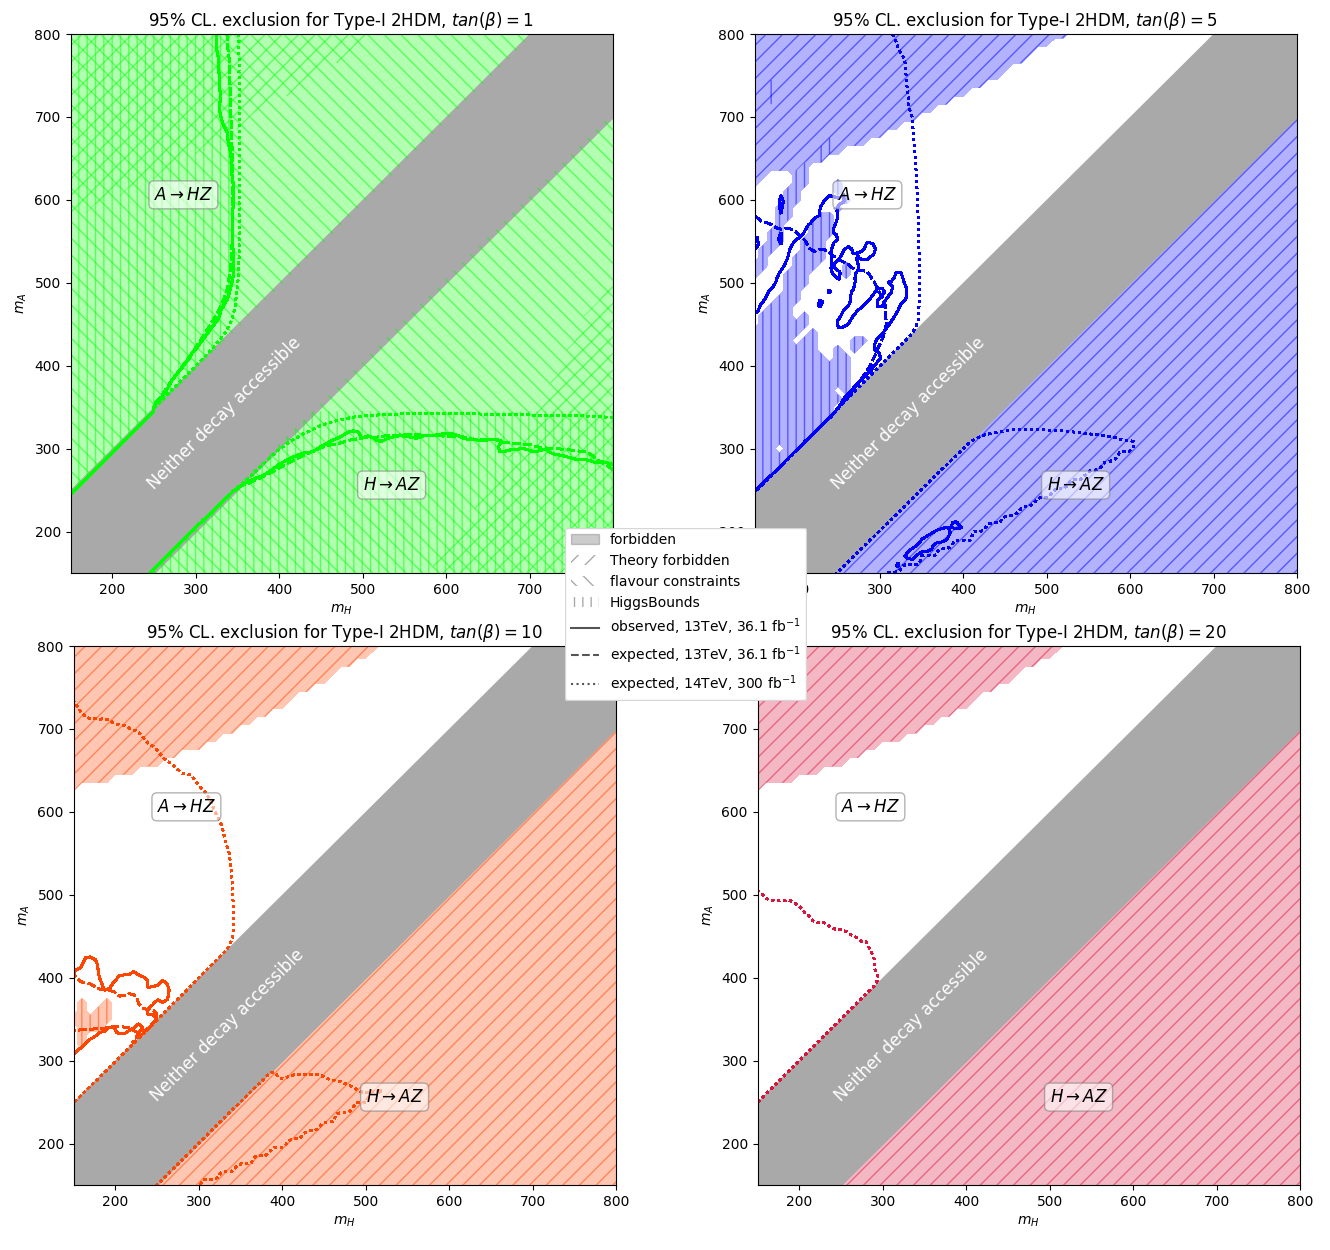
\includegraphics[width=\textwidth]{single_tbs/type1.png}
    \caption{Exclusion limits at \(95\%\) CL in Type-I.
             The lines denoting expected and observed exclusion limits
             do not appear at all on some plots when the prediction never exceeds the 
             expected or observed  limit.}\label{fig:2HDMparams1}
\end{figure}

\begin{figure}[t!]		
    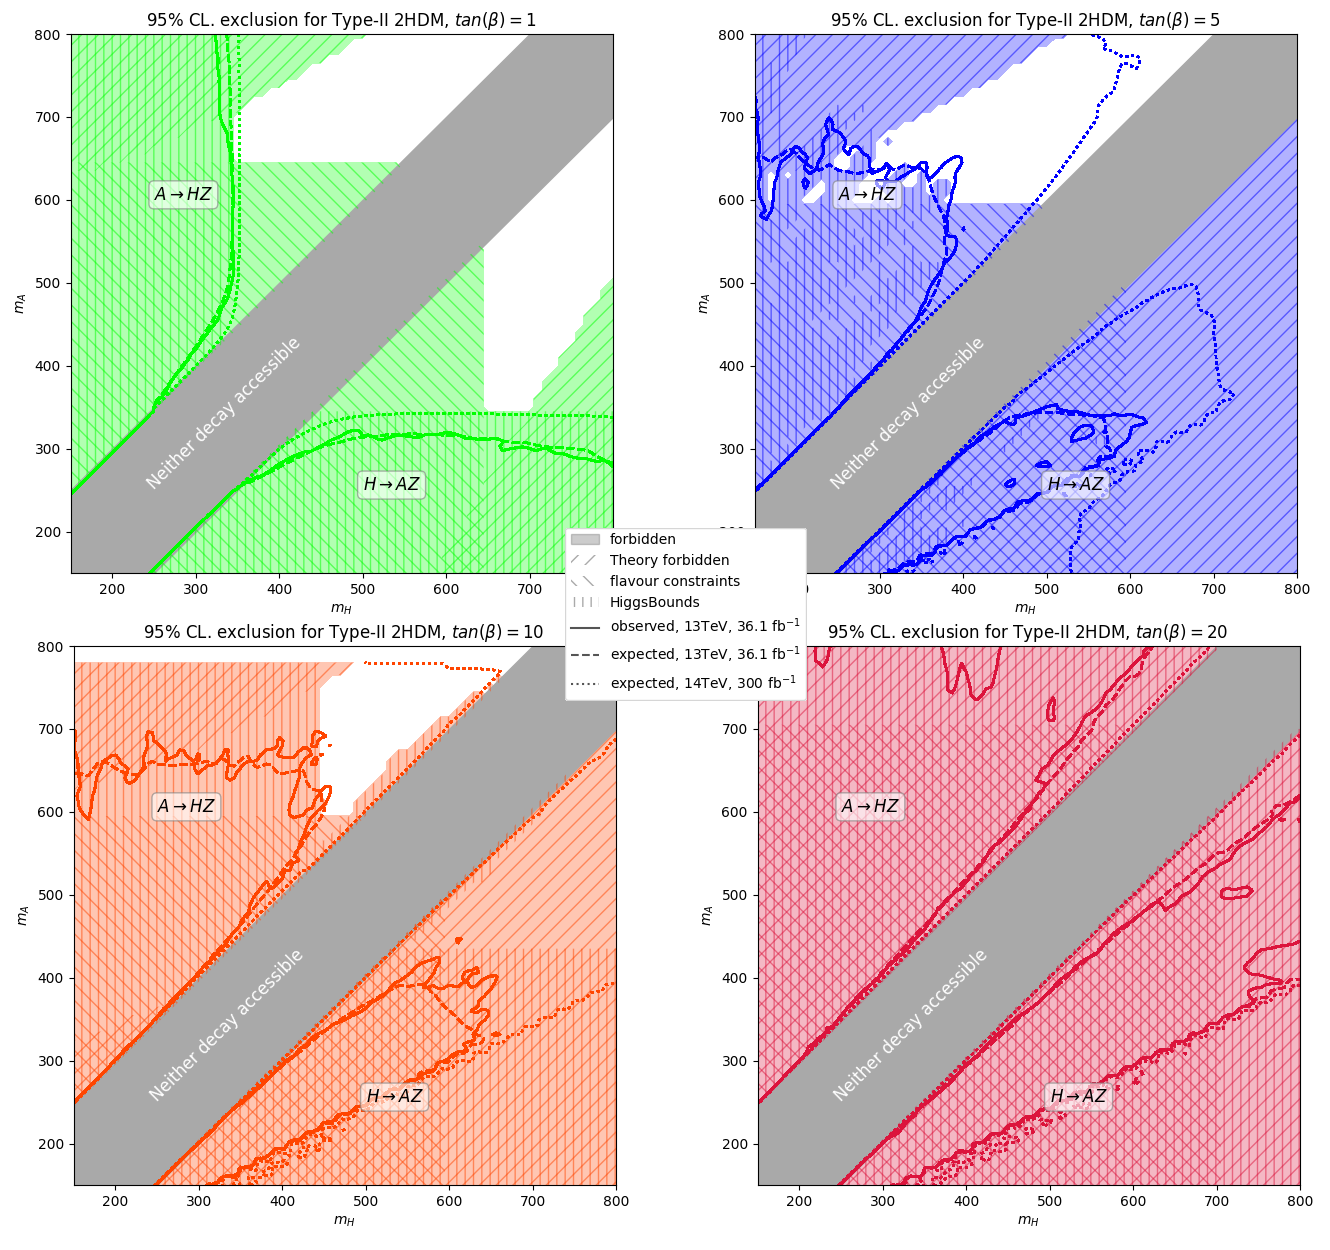
\includegraphics[width=\textwidth]{single_tbs/type2.png}
    \caption{Like in Fig.~\ref{fig:2HDMparams1} but for Type-II.}\label{fig:2HDMparams2}
\end{figure}


\begin{figure*}[t!]	     
    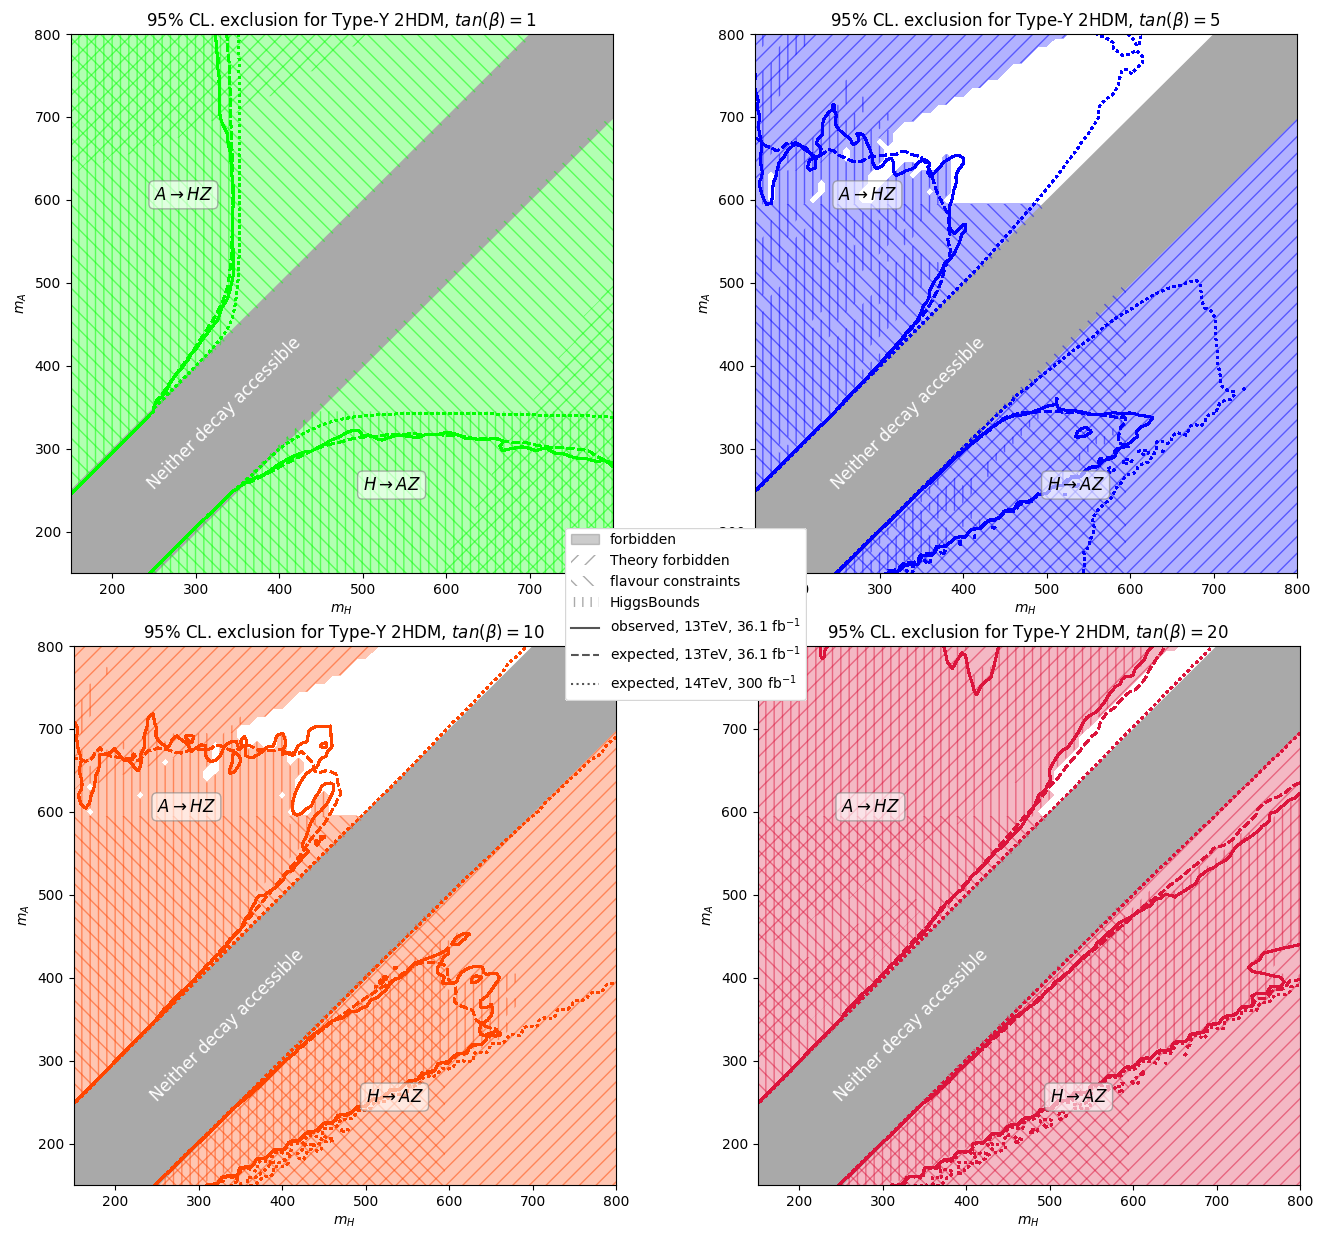
\includegraphics[width=\textwidth]{single_tbs/type3.png}
    \caption{Like in Fig.~\ref{fig:2HDMparams1} but for Type-Y (Flipped).}\label{fig:2HDMparams3}
\end{figure*}

\begin{figure*}[t!]
	\centering
    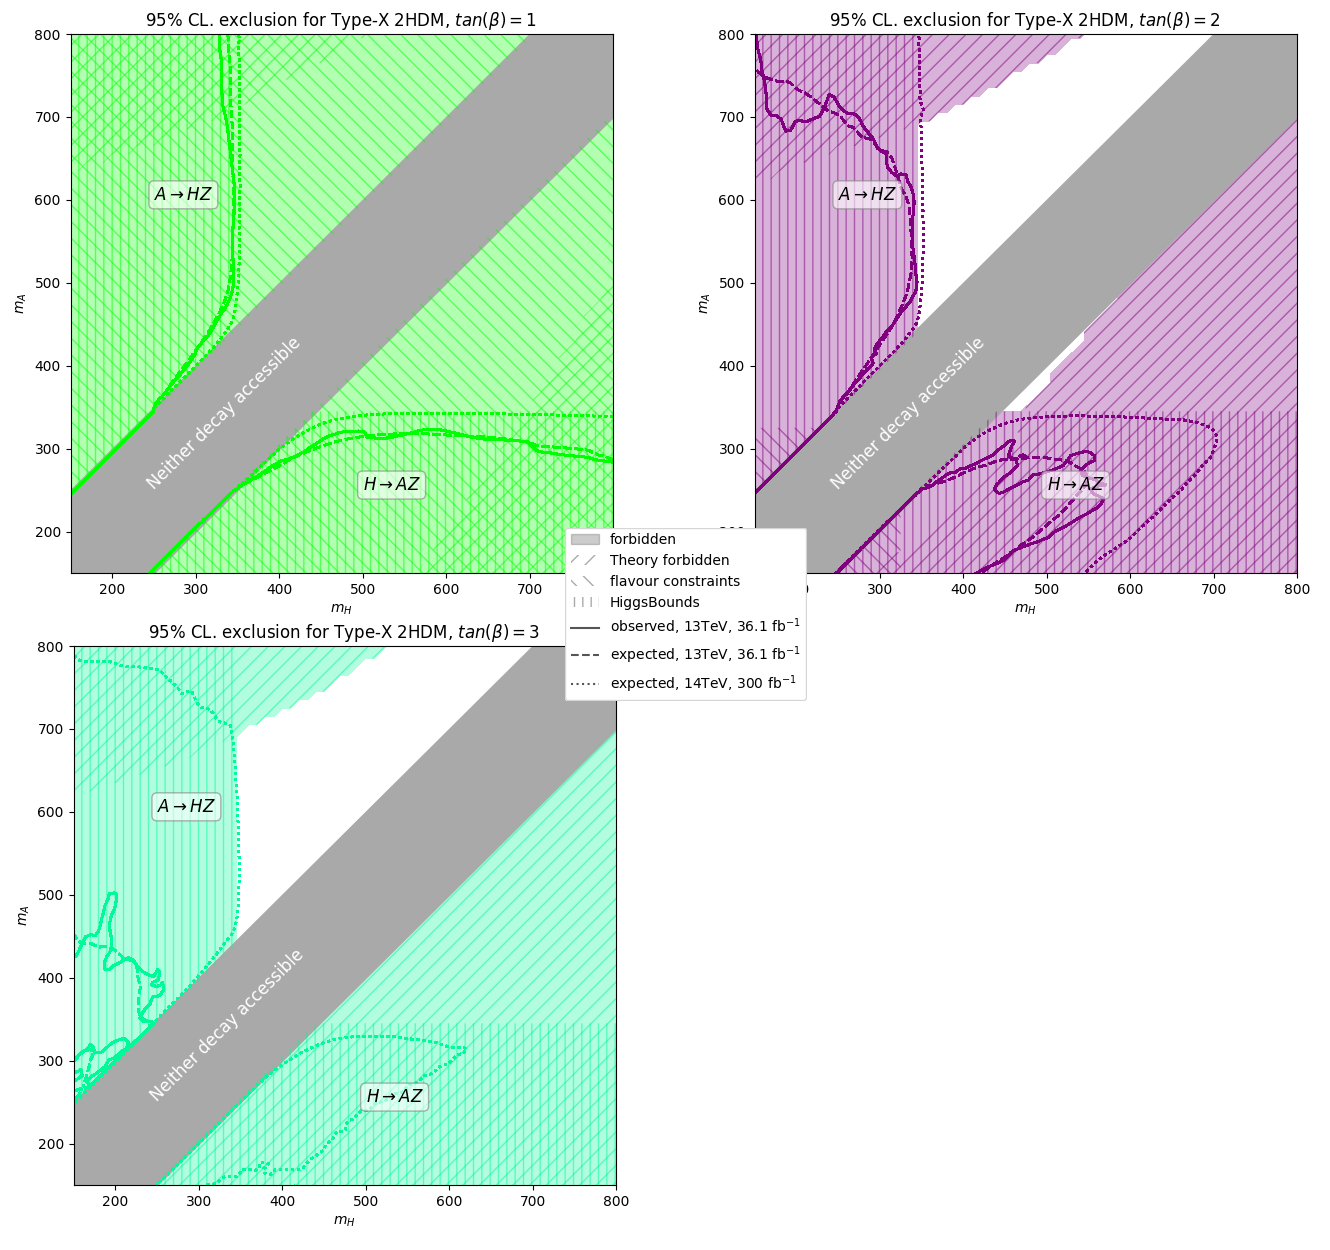
\includegraphics[width=\textwidth]{single_tbs/type4.png}
    \caption{Like in Fig.~\ref{fig:2HDMparams1} but for  Type-X (Lepton specific).}\label{fig:2HDMparams4}
\end{figure*}

While an evident symmetry exists between the two cases, neither the constraints affecting the two processes nor their  sensitivity reaches should be expected to be symmetric.
On the one hand, the role played by the heavy CP-even and CP-odd Higgs states of the 2HDM in both theoretical and experimental limits is different, owing to their different quantum numbers (and hence couplings).
On the other hand, their production and decay rates at the LHC are different despite leading to the same final states, including residual differences due to width effects entering their normalisation (but, as mentioned, not their kinematics), since, e.g., the $A$ state does not decay to $W^+W^-$ and $ZZ$ pairs while the $H$ state does and, conversely, the $A$ state decays to $Zh$ while the $H$ state does not.  
However, in the alignment limit used here these decay channels are closed.
\subsubsection{Theoretical constraints}
Within these ranges there are several theoretical and experimental constraints for the parameter points of the 2HDM to pass, discussed below.	
\begin{itemize}
	\item Unitarity: various scattering processes  require that unitarity is conserved at the tree-level at high energy.
    The unitarity requirements in the 2HDM have been studied in~\cite{Kanemura1993LeeQuiggThacker, Akeroyd2000TreeLevel, arhrib2000unitarity}.
	%Sets of eigenvalues $e_i$ ($i-1, ... 12$) for the scattering  matrix of all Higgs and Goldstone bosons of the 2HDM are obtained as follows:
	%\begin{eqnarray}
	%&& e_{1,2} =  \lambda_3+2\lambda_4\pm 3 | \lambda_5| , \quad  \quad  e_{3,4} = \lambda_3\pm\lambda_4 , \quad e_{5,6} =  \lambda_3\pm|\lambda_5|,  \nonumber \\
	%&&
	%e_{7,8} = 3(\lambda_1+\lambda_2)\pm\sqrt{9(\lambda_1-\lambda_2)^2+4(2\lambda_3+\lambda_4|)^2},  \nonumber \\
	%&&
	%e_{9,10} = \lambda_1+\lambda_2\pm\sqrt{(\lambda_1-\lambda_2)^2+4|\lambda_5|^2},  \nonumber \\
	%&&
	%e_{11,12}  = \lambda_1+\lambda_2\pm\sqrt{(\lambda_1-\lambda_2)^2+4|\lambda_5|^2}.
	%\end{eqnarray}
    %We require all \(e_i\)'s to be less than 16\(\pi\) for each \(i=1,...12\).
%\item Perturbativity constraints \cite{Kanemura1993LeeQuiggThacker,Branco_2HDMreview2011} implies that all that the quartic couplings of the scalar potential satisfy the condition \(|\lambda_i| \leqslant 8 \pi\) for each \(i=1,...5\).
\item Perturbativity constraints are given in ~\cite{Kanemura1993LeeQuiggThacker,Branco_2HDMreview2011}.
	
	\item Vacuum stability requires the scalar potential to be bounded from below~\cite{Gunion2003decouple}.% by satisfying the following inequalities:
	%\begin{eqnarray}
	%\lambda_{1,2}>0,  \,\,
	%\lambda_3>- \sqrt{\lambda_1\lambda_2}, \,\,
	%\lambda_3+\lambda_4-|\lambda_5|> - \sqrt{\lambda_1\lambda_2}.~~~
	%\end{eqnarray}
	
\end{itemize}
In practice the theoretical constraints are automatically checked by the program 2HDMC~\cite{Eriksson20102HDMC}.
The program can determine if a selected parameter combination is valid.

The choice of \(m^2_{12} = m_A^2 \tan(\beta) / (1 + \tan(\beta))^2\) enables us to reconstruct the exclusion limits at 95\%  confidence level (CL) given in Ref~\cite{Aaboud2018AZHbbll}.
However, this choice does not actually allow to satisfy theoretical constraints in all four types of 2HDM.
In contrast, our choice of \(m_{12}^2\) above aims to simultaneously satisfy as many theoretical constraints as possible while affording one with significant parameter space amenable to experimental investigation.

2HDMC is a well engineered, fast library;
however owing to the range of possible values in \(m_{12}^2\) some curve fitting of the valid points
is required to augment the MC sampling.
Points that satisfy the most constraints are fitted to a polynomial and
values of \(m_{12}^2\) near the surface of the polynomial are sampled further.

\subsubsection{Experimental constraints}
In addition to theoretical constraints experimental constrains need to be accounted for.
\begin{itemize}
	\item EW Precision Observables (EWPOs) \cite{Haller2018EWUpdate}, such as the oblique parameters $S$ and $T$ \cite{Peskin:1991sw, Grimus2008Oblique}, require a level of degeneracy between the charged Higgs boson state and one of the heavier neutral Higgs bosons. Here, we assume $m_{H^\pm} = m_{A}$  or $m_H$, as appropriate (see below), so that the $T$ parameter exactly vanishes in the alignment limit. 
    \item Exclusion limits at 95\% CL from Higgs searches at colliders (LEP, Tevatron and LHC) via HiggsBounds, version 5.3.2~\cite{Bechtle2009higgsbounds, Bechtle2011higgsbounds2, Bechtle2014higgsbounds4} are enforced.
    Furthermore, the ATLAS Collaboration has set an upper limit at 95\% CL on the production cross section $\sigma$ of the $A$ state times its decay BR into $ZH\to l^+l^-b\bar b$, i.e., \(\sigma(A)\times {\rm BR}(A\rightarrow ZH \rightarrow l^+l^-b\bar b)\)~\cite{Aaboud2018AZHbbll}, that is not included in this tool, hence we have accounted for it separately.
	
\item Constraints from the Higgs boson signal strength measurements are automatically satisfied as we assume $\sin(\beta-\alpha) =1$.	
	
\item Constraints of {flavour physics observables,} namely, \(B \rightarrow X_s \gamma,~ B_{s,d} \rightarrow \mu^+\mu^-\) and \(\Delta m_{s,d}\)~\cite{Haller2018EWUpdate}.		
\end{itemize}

Comparing to observed and expected exclusion limits requires obtaining branching ratios and production cross sections.
The relevant branching ratios, \AZH{}, \HZA{}, \Abb{} and \Hbb{} are calculated with 2HDMC~\cite{Eriksson20102HDMC}.
The production cross sections of the heavy CP-even ($H$) and CP-odd ($A$) Higgs bosons,
at Next-to-Next-to-Leading Order (NNLO) in QCD, 
for both $gg\to H,A$ and $b\bar b\to A,H$, at the Centre-of-Mass (CM) energies of 13 TeV and 14 TeV,
are calculated using SusHi~\cite{Harlander2013SusHi, Harlander2017Bento, Harlander2002nexttonext, Harlander:2003ai}. 
Of all the calculations required for the scan this one required most compute time,
therefore some optimisations to the code were investigated.
Firstly, much of the compute time was on unneeded disk reading and writing,
this was circumnavigated by piping the input and output,
such that the data that would have gone to the disk stayed in the ram.
This produced a \(30\%\) speed increase.
Secondly, the program was not natively vectorised.
To allow the computation to be done in parallel without race conditions
and with minimal possibility of introducing a new bug
a python script to split in input and launch the program in multiple,
non interacting, threads was developed.

2HDMC code also includes an interface to HiggsBounds, which is used to apply the aforementioned exclusion limits at 95\% CL from Higgs searches at LEP, Tevatron and LHC.

The first part of this study deals with the two production and decay processes \(pp \rightarrow H(A) \rightarrow ZA(H)\rightarrow b\overline{b}l^{-}l^{+}\).
The observed and expected confidence limits for all four types of Yukawa couplings in the 2HDM are produced at \(\sqrt{s}=13\)~TeV, with an integrated luminosity, $L$, of \(36.1~{\rm fb}^{-1}\),
by combining our calculations with the data from Ref.~\cite{Aaboud2018AZHbbll}. 
In the second part, we rescale the expected exclusion limit to the CM energy of \(\sqrt{s}=14\)~TeV,
with an integrated luminosity of \(300~{\rm fb}^{-1}\), by calculating the so called `upgrade factor' for both signals and backgrounds, while retaining the acceptance and selection efficiencies of the analysis at the lower $\sqrt s$ value. The change in energy will naturally affect signals and backgrounds differently. We treat the former by using SusHi (as intimated) and the latter by  using {MadGraph5, version 2.6.4}~\cite{alwall_madgraph2011}. (For completeness, the
 background is considered to be any reducible or irreducible SM process that creates a pair of $b$-jets plus a pair of electrons or muons, as in Ref.~\cite{Aaboud2018AZHbbll}.)

\subsection{Numerical results}


%\begin{figure*}[t!]
%	\centering
%    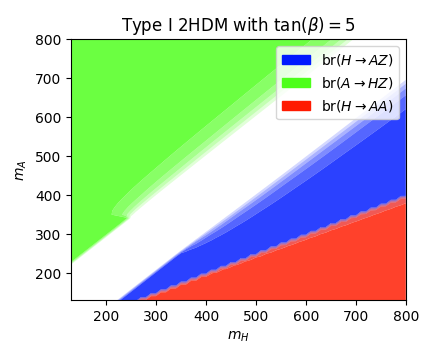
\includegraphics[width=.5\textwidth]{branching_ratios_HAA.png}
%    \caption{The branching ratio \(H\rightarrow AZ\) is suppressed by the branching ratio \(H\rightarrow AA\).
%             This effect occurs for all types, but does not occur at small \(\tan(\beta)\).}\label{fig:2HDMparamssuppress}
%\end{figure*}

After performing a scan over the parameter space delimited by Eq.~(\ref{eq1}), we compare the prediction of the model with the observed and expected limits given in Ref.~\cite{Aaboud2018AZHbbll}.
If the prediction exceeds the observed limit, then the parameter combination is excluded.
When the prediction exceeds the expected limit, we anticipate that the signal would be visible above background given the energies and luminosities available, hence,  {the experiment is sensitive to these parameters.} %these parameters are testable.


Figs.~\ref{fig:2HDMparams1}~to~\ref{fig:2HDMparams4} illustrate the outcome the scan for each
Yukawa type, \(\tan(\beta)\) and mass combination $(m_H,m_A)$.
Each figure provides results for one choice of Yukawa couplings
and each frame in each figure provides results at one value of \(\tan(\beta)\).
In the top left of each plot, where \(m_A > m_H+100\)~GeV, the decay \AZH{} is considered while 
in the bottom right of each plot, where \(m_H > m_A+100\)~GeV,   the decay \HZA{} is considered.
The corridor along the diagonal between these regions is coloured grey to indicate that neither decay is accessible.
%
If a combination of parameters is forbidden by theory, HiggsBounds or flavour constraints
then the corresponding area is filled with solid colour, conversely,
white areas pass all these checks and so are of interest. The hatching over the solid colour is used to indicate which of the checks
causes the corresponding parameter combination to fail.
There are three boundary lines drawn over the plots: 
these are the observed and expected \(95\%\) CLs for the ATLAS detector in its present state, \(13\) TeV and \(36.1~\text{fb}^{-1}\),
plus the expected 95\% CL for an upgraded LHC and ATLAS detector at \(14\) TeV and \(300~\text{fb}^{-1}\)\footnote{We neglect here to consider the case of $\sqrt s=13$ TeV and $L\approx140$ fb$^{-1}$, as it only improves marginally the present situation yet it would be make the plots far too crowded.}.
The model predictions exceed the 95\% CL inside the curve.


\begin{table}
\begin{tabularx}{\textwidth}{RCCCC}
      \toprule
      \textcolor{black}{\(\tan(\beta)\)}& \textcolor{black}{\(1\)} & \textcolor{black}{\(5\)} & \textcolor{black}{\(10\)} & \textcolor{black}{\(20\)}\\
      \toprule
      Type-I & \textcolor{red}{Flavour constraints} & \textcolor{blue}{Some masses} & \textcolor{blue}{Many masses} & \textcolor{red}{Low sensitivity} \\
      \hline
      Type-II &\textcolor{red}{Flavour constraints} & \textcolor{blue}{Some masses after upgrade} & \textcolor{blue}{Some masses after upgrade} & \textcolor{red}{Theory constraints}\\
      \hline
      Flipped &\textcolor{red}{Flavour constraints} & \textcolor{blue}{Some masses after upgrade} & \textcolor{blue}{Some masses after upgrade} & \textcolor{red}{Theory constraints}\\
      \toprule
      \textcolor{black}{\(\tan(\beta)\)}& \textcolor{black}{\(1\)} & \textcolor{black}{\(2\)} & \textcolor{black}{\(3\)} & \\
      \toprule
      Lepton specific & \textcolor{red}{Flavour constraints} & \textcolor{red}{Excluded by HiggsBounds} &  \textcolor{red}{Excluded by HiggsBounds} & \\
\end{tabularx}
%\vspace*{-1cm}
\caption{Table summarising the findings in Figs.~\ref{fig:2HDMparams1}~to~\ref{fig:2HDMparams4}.
An overview of the possibility of each Yukawa type and value of \(\tan(\beta)\) is given.
Entries in red indicate that the combination has little or no mass combinations that are not forbidden while those in blue represent available parameter space accessible presently at Run 2  or after the upgrade of Run 3.}
\label{tab:summary}
\end{table}


\subsection{Conclusions}
In summary, we have revisited an experimental analysis of the ATLAS Collaboration of the production and decay process $gg,b\bar b\to A\to ZH\to l^+l^-b\bar b$ performed at Run 2 with 36.1 fb$^{-1}$ of luminosity, which had been interpreted in terms of exclusion limits over the parameter space of the four types of the 2HDM, wherein the lightest Higgs state is identified with the SM-like Higgs boson discovered during Run 1 at the LHC with mass 125 GeV. Upon validating the ATLAS interpretation in our framework, though, we have discovered that their (fixed) choice of $m_{12}$, a mass parameter in the 2HDM Lagrangian that softly breaks an underlying $Z_2$ symmetry of the 2HDM to avoid FCNCs, yields parameter space configurations which are ruled out by theoretical requirements of model consistency. Hence, we have allowed this parameter to vary freely and subject the ensuing parameter space configurations to both the aforementioned theoretical constraints as well as those emerging from past and present experiments, thereby redrawing the actual sensitivity of such an experimental search to all four Yukawa types of the 2HDM, as a function of $\tan(\beta)$. In doing so, we have have also forecast the potential sensitivity of this channel to the 2HDM parameter space at the end of Run 3, assuming increased energy to 14 TeV and luminosity to 300 fb$^{-1}$.
This revealed some extended coverage of the 2HDM Type-I, -II and -Y (but not -X),
especially for intermediate $\tan(\beta)$ values (say, between  5 and 10), with $m_A$ up to 800 GeV and $m_H$ up to 700 GeV.
This is somewhat beyond what is presently covered, i.e.,  up to 150 GeV or so in mass of either Higgs state, so as to justify further searches for this signature at the next stage of the LHC. Finally, we have recast the sensitivity of this analysis onto that of the channel  $gg,b\bar b\to H\to ZA\to l^+l^-b\bar b$. However, we have found that the complementary parameter space accessible this way (i.e., $m_H\ge  m_A+m_Z$) is actually entirely excluded already by existing theoretical and/or experimental constraints, so as to conclude that it is not warranted to pursue further this channel at the LHC, at least, not with a view to interpret it in the context of the standard four Yukawa types of the 2HDM\footnote{We finally note that analyses similar to Ref.~\cite{Aaboud2018AZHbbll}
performed by the CMS Collaboration exist \cite{Khachatryan2016resonancesbbtautau,Sirunyan2020newneutral}. We have not used these for two reasons. On the one hand, they did not convey all the  information necessary to make  extrapolations to higher energies. On the other hand, they did not afford one with significantly different sensitivity to the 2HDM at present energies than what achieved by the ATLAS analysis ~\cite{Aaboud2018AZHbbll} that we have adopted as benchmark.}.


    \FloatBarrier
    \section{Jet Clustering}\label{sec:JetClustering}
This next section considers a completely novel approach to jet clustering, spectral clustering.

As mentioned previously, the default choice for jet clustering tends to be one of there algorithms;
the anti-kt algorithm~\cite{Cacciari2008akt}, the Cambridge-Aachen algorithm~\cite{Wobisch1998caJet} and the kt algorithm~\cite{Ellis1993ktJet}.
They have been the default choice for some time because they have a number of desirable properties.
They are infrared safe, excellent implementations of them are available (see \fastjet{}~\cite{Cacciari2011FastJet})
and it is flexible enough to capture many signals with minimal parameter change.
These algorithms are recursive and agglomerative.
A recursive algorithm is well suited to clustering objects when the number of groups is not known at outset.
Agglomerative algorithms are easier to design in a manner that is infrared safe,
as they can recombine soft and collinear emissions in early steps.

Finding a clustering method that compares favourably to these algorithms is challenging.
Spectral clustering is a candidate that has had considerable success in other studies.
In fluid dynamics spectral clustering has been used to identify the motion
of vortices~\cite{hadjighasem2016votex}, finding that it is possible
to successfully identify the vortex structures in cases with less data available.
It was also seen that spectral clustering was proficient at determining the correct number
of clusters to be found in the fluid.
To reduce the risk of blackouts, power grids may be subdivided into `islands'.
The ideal allocation is found by minimising power flow between islands,
and it was shown in~\cite{fennelly2014power} that spectral clustering
can produce a good solution in less time than other algorithms commonly used for this problem.

%Adaptive spectral clustering with application to tripeptide conformation analysis~\cite{haack2013AdaptiveSC}.  %TODO

To the authors knowledge this clustering algorithm has not yet been applied to jet physics, %TODO - double check.
however, given its recursive, agglomerative form it could be a good fit.

    \FloatBarrier
    \section{Theory of spectral clustering}\label{sec:spectral_theory}

Collimated emissions of particles are clustered by jet algorithms.  A
representation of observable particles that preserves and accentuates local information
motivates the Laplacian eigenmap~\cite{BelkinNiyogi2003} and spectral
clustering~\cite{NgJordanWeiss2002}.
Spectral clustering is a method by which a set of points are represented in a new space,
called the embedding space, in which they can be easily clustered.  Coordinates of the
points in the embedding space are expressed in terms of the eigenvectors and eigenvalues
of an associated Laplacian matrix, hence the name.

The particles in an event are described first as nodes of a graph and
edges capturing a notion of similarity between them.
The theory behind the
construction of the embedding space is a relaxation of criteria that would precisely
partition nodes into separate disconnected subgraphs.
An excellent description can be found in~\cite{luxburg2007spectraltutorial}; a short
summary is given here.

At the start we have a group of points with coordinates, which should be split into a  number \(c\) of predetermined clusters.
Applying the spectral clustering method requires making these points into a graph.
A simple way to do this would be to consider the points to be the nodes of a fully connected graph.
The vertex of the graph joining node (or point) \(i\) and \(j\) has weight \(a_{i, j}\),
which should grow with the probability of \(i\) and \(j\) being in the same group.

The initial aim is to identify which of the components each point belongs to,
by sorting the graph into subgraphs, \(G_k\), where \(k=1 \dots c\).
Minimising the NCut objective is a function that captures this aim, where 
\begin{equation}
    \text{NCut} = \frac{1}{2}\sum_k\frac{W(G_k, \bar{G_k})}{\text{vol}(G_k)},
\end{equation}\label{eqn:cost_function}
where \(W(G_k, \bar{G_k})\) is the sum of all the vertex weights that must be dropped
to separate the cluster \(G_k\) from the rest of the graph, \(\bar{G_k}\).
So that \( W(G_k, \bar{G_k}) = \sum_{i \in G_k, j \in \bar{G_k}} a_{i, j} \).
In the denominator \(\text{vol}(G_k) = \sum_{i \in G_k} \sum_{j} a_{i, j}\),
the sum of all affinities connecting to a point in \(G_k\).
This denominator is used to penalise forming small clusters.

In order to determine which point will go in which \(G_k\), a set of indicator vectors must be found.
Membership of cluster \(G_k\) will be recorded in the indicator vector \(h_k\):
\begin{equation}\label{eqn:indicator}
    h_{i, k}= 
    \begin{cases}
        1/\sqrt{\text{vol}(G_k)}& \text{if point } i \in G_k ,\\
        0             & \text{otherwise},
    \end{cases}
    .
\end{equation}

To find these indicator vectors the graph is represented by the graph Laplacian, \(L\), a square
matrix with as many rows and columns as there are points.
To construct this Laplacien we define two other matrices;
an off diagonal matrix 
\(A_{i, j} = (1 - \delta_{i, j})a_{i, j}\)
and a diagonal matrix
\(D_{i, j} = \delta_{i, j}\sum_q a_{i, q}\).
Then the symmetric Laplacian can be simply written as;
\begin{equation}\label{eqn:symmetric_laplacian}
    L = D^{-\frac{1}{2}} (D - A) D^{-\frac{1}{2}}
\end{equation}

Notice that this is a real symmetric matrix
and, therefore all its eigenvalues are real.
Considering just one cluster, \(G_k\), when the Laplacian is multiplied by its indicator vector,
the result is the term that NCut seeks to minimise for that cluster.
\begin{equation}
    h_k'Lh_k = \frac{1}{\text{vol}(G_k)}\sum_{i \in G_k, j \in G_k} \left(\delta_{i, j}\sum_{l} a_{l, i} - a_{i, j} \right) = \frac{W(G_k, \bar{G_k})}{\text{vol}(G_k)}
\end{equation}
To obtain the sum of all the terms, stack the indicator vectors into a matrix,
\( h'_k L h_k = (H'L H)_{kk}\),
and the NCut aim described earlier becomes the trace,
\begin{equation} \text{NCut}(G_1,G_2, \dots G_n) \equiv \frac{1}{2} \sum_{k=1}^n \frac{W(G_k, \bar{G_k})}{\text{vol}(G_k)} = \text{Tr}(H'LH),\end{equation}
where \(H'H = I\).
This is still an NP hard problem, however if we relax the requirements made on \(h\) in Eqn.~\ref{eqn:indicator},
allowing the elements of \(h\) to take arbitrary values, then the Rayleigh-Ritz theorem provides a solution.
Trace minimisation in this form is done
by finding the eigenvectors of \(L\) with smallest 
eigenvalues.
Due to the form of the Laplacian, there will be an eigenvector with components all of the same value and its eigenvalue will be \(0\).
This corresponds to the trivial solution of considering all points to be in one group.
The next \(c\) eigenvectors of \(L\), sorted by smallest eigenvector, are the indicator vectors needed to allocate points to \(c\) clusters.

These indicator vectors are then used to determine position of the points in the embedding space.
Each indicator vector has as many elements as there are points to be clustered,
so the coordinates of a point are the corresponding elements or the indicator vectors.
This is all the information the theory of spectral clustering provides.
The steps required to make use of this information are not dictated by the theory,
and they must be carefully selected to respect the physics.

Using the positions in embedding space the points can be gathered agglomeratively,
so that we do not need to chose a predetermined number of clusters.

\subsection{Distance in the embedding space}\label{sec:embedding_distance}
When the relaxed spectral clustering algorithm is used to create an embedding space, points in a group will not be at exactly the same coordinates.
Each point can be seen as a vector, the direction of this vector indicates the group to which this point should be assigned.
The magnitude indicates the confidence with which the assignment is made.
Changes in magnitude cause the Euclidean distance between the corresponding points to grow.
An angular distance is appropriate, though. 
The angular distance will grow when the eigenvectors indicating the point have less overlap
and this is what should be measured.

\subsection{Information in the eigenvalues}\label{sec:eig_norm}
When the clusters in the data are very clear, the situation is closer to the ideal one and the eigenvalues will be closer to \(0\).
The smaller an eigenvalue is, the more like a perfect indicator vector the corresponding eigenvector is.
It is possible to make use of this information.

In a traditional application of spectral clustering, the number of clusters desired, \(c\), is predetermined.
The embedding space is created by taking \(c\) eigenvectors with smallest eigenvalues, excluding the trivial eigenvector.
The embedding space then has \(c\) dimensions.
This follows from a relaxation of the concept of indicator vectors.

When forming jets we do not know from the outset how many clusters to expect in the dataset,
so the number of eigenvectors to keep is not clear.
While we could chose a fixed, arbitrary number of eigenvectors, this is suboptimal.
A better approach is to take all non-trivial eigenvectors corresponding to eigenvalues
smaller than some limiting number, \(\lambda_\text{limit}\).
For a symmetric matrix the eigenvalues will be \(0 < \lambda < 2\),
so \(\lambda_\text{limit} = 0.5\) would be a reasonable choice.
Then, the number of dimensions in the embedding space will vary,
according to the number of non-trivial eigenvectors with corresponding \(\lambda < \lambda_\text{limit}\).

There is one more manipulation from the information in the eigenvalues.
The dimensions of this embedding space are not of equal importance,
those with higher eigenvalues being less interesting.
This can be accounted for by dividing the eigenvector by some power, \(\beta\), of the eigenvalue.

Let the eigenvectors for which \(\lambda < \lambda_\text{limit}\) be
\begin{equation}
    L_{i, j} (h_n)_j = \lambda_n (h_n)_i.
\end{equation}
Then, the coordinates of the \(j^\text{th}\) point in the \(c\) dimensional embedding space
become \(m_j = \left(\lambda_1^{-\beta} (h_1)_j, \dots \lambda_c^{-\beta} (h_c)_j,\right)\).
In effect the \(n^\text{th}\) dimension is compressed by a factor \(\lambda_n^\beta\),
so the larger \(\lambda_n\) the greater the compression.

\subsection{Stopping conditions}\label{sec:stopping_condintion}

If a recursive algorithm is to be chosen, like in the \genkt{} algorithm, a stopping condition is needed.
A stopping condition based on smallest distance between points in the embedding space does not prove to be stable,
as the distribution  in the number of dimensions in the embedding space changes sharply from event to event.

The average distance between points is more stable.
If this were used in physical space it would force roughly the same number of clusters to form each time,
however, the variable number of dimensions in the embedding space is now an advantage.
The  clearer information found about clusters in the points the more dimensions the embedding space will contain,
as described in section~\ref{sec:eig_norm}.

Say, the data contains two points that would form a good cluster.
If those two points are combined into one, that cluster is complete,
fewer clusters remain unfinished
and the information for clustering the resulting points will be reduced.
When the embedding space is recalculated for the new points, it will likely have fewer dimensions.
In a space with fewer dimensions the mean distance between the points naturally falls.
Thus, the mean distance in the embedding space is a good indicator of the number of unfinished clusters available.
In short, the mean distance in the embedding space makes a natural cut-off.

    \FloatBarrier
    \subsection{Method}
\subsubsection{Particle data}
The dataset used for the majority of this work is a simulated Higgs cascade decay.
One Standard Model (SM) Higgs at \(125\)GeV decays to two light Higgs at \(40\)GeV,
which in turn decay to \beau{}-\bbar{} quark pairs.
That is \(H_{125\text{GeV}} \rightarrow h_{40\text{GeV}} h_{40\text{GeV}} \rightarrow \beau \bbar \beau \bbar\).


This dataset has the desirable property of creating \bthing{jets} with a range of geometries
owing to the boost provided by large mass of the SM Higgs and
the high chance of overlap with 4 \bthing{quarks} in the event.
Other radiation from the protons is also included.  % TODO clarify exactly what background is in here!


Before any evaluation can be performed on the final state of the simulation
particles that ended outside the range of the silicon tracker (\(|\eta|>2.5\))
or particles with low transverse momentum (\(p_T < 0.5\) GeV) are cut.
This is to mimic restrictions from reconstruction accuracy.

\begin{figure}[htp]
    \begin{minipage}[c]{0.5\textwidth}
        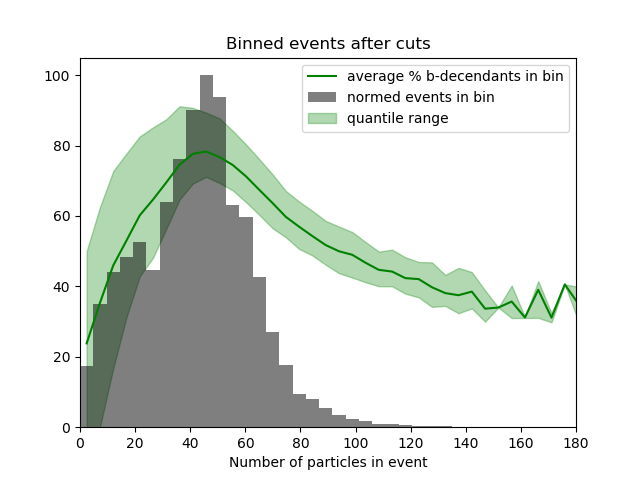
\includegraphics[width=1\textwidth]{graphics/binned_events.png}
    \end{minipage}\hfill
    \begin{minipage}[c]{0.45\textwidth}
        \caption{The end state particle in the simulated events are filtered
            with the standard cuts, \(p_T > 0.5\), \(|\eta| < 2.5\).
            The events are binned according to how many particles remain after the cuts.
            The percentage of \bthing{descendants} in the remaining event after the cuts
            is averaged for each bin and plotted on the same axis.
            After the cuts have been applied most events are left with around \(50\) particles.
                 The percentage of particles that are descendant from a \bthing{quark} varies,
                 it is at it's highest in events with \(50\) particles,
             and most variable in events will small multiplicity.}\label{fig:bdecendantpercent}
    \end{minipage}
\end{figure}    

A particle is considered a \bthing{descendant} if is found in the chain of decays from a \bthing{quark}.
After cuts, \(72\%\) of events have at least \(5\) \bthing{descendants} and \(5\) non \bthing{descendants} available.
Exactly how the percentage of \bthing{descendants} changes with event size is visualised in figure~\ref{fig:bdecendantpercent}.

\subsubsection{Clustering algorithm}\label{sec:spectralmethodalgo}
Now the implementation of the theory described in section~\ref{sec:spectral_theory} will be specified.
For every simulated event this process if used to select a clustering.

\begin{enumerate}
    \item \label{step:start} The particles are to be used to form the nodes of a graph,
    the edges of which will be weighted by some measure of proximity between the particles known as affinity.
    To obtain an affinity, first a distance is obtained; \(d_{i,j} = \sqrt{(y_i - y_j)^2 + (\phi_i - \phi_j)^2}\)
    where \(y_i\) is the rapidity of particle \(i\) and \(\phi_i\) is the barrel angle is particle \(i\).

    \item The distance shrinks as particles become similar, to obtain an affinity this must be transformed so that
    the value grows with increasing similarity.
    This is done by taking an inverse so that \(a_{i,j} = 1/d_{i,j}\), as done in~\cite{hadjighasem2016votex}. % TODO check you stick with this

    \item These affinities allow the construction of a Laplacien.
    The Laplacien used is the unnormalised Laplacien, which has \(\sum_j a_{i,j}\) in the \(i\)th
    diagonal entry (also known as the degree of node \(i\)) and \(-a_{i,j}\) of the diagonal 
    in column \(i\) row \(j\).

    \item From the Laplacien a predetermined number of eigenvectors are calculated to create the embedding space.
    The eigenvectors have as many elements as there are particles, and the coordinates of
    the \(i\)th particle in the embedding space is the \(i\)th element of each eigenvector.

    \item The first clustering can be done based on 
    a measure of distance derived from the particles \(p_T\) and it's position in the embedding space.
    The \(p_T\) is used as in the Luclus~\cite{moretti1998new}, with a variable exponent, \(q\);
    \[p_T \text{ factor} = \left(\frac{{p_T}_i{p_T}_j}{s({p_T}_i+{p_T}_j)}\right)^q\].
    Where \(s\) is the invariant mass of all observed particles in the event, it is used
    to make the \(p_T\) factor unitless.
    The embedded distance is euclidean distance in the embedding space multiplied by this factor.

    \item The two object that have the smallest embedding distance are combined.
    In physical space the combined object is created by summing the respective four momenta,
    in the embedding space two methods for locating the combined object are tried.
    \begin{enumerate}
        \item In a \spectralmeanjet{} clustering the location of the combined object is the
        geometric mean of the inputs. The clustering then continues to combine things in this manner.
        \item In a \spectralfulljet{} once two object have been combined in physical space
            the embedding space is recalculate from step~\ref{step:start}. 
    \end{enumerate}

    \item When the closest object to a particle in the embedding space is further away than \stoppingdeltar{}
    then the combined object is considered to be a complete jet and removed from future clustering.
\end{enumerate}
To provide a basis for comparison the results of clustering with an anti-kt algorithm (as in~\cite{Cacciari2008akt}) is also shown.


    \FloatBarrier
    \section{Results}

Before the behaviour of the algorithms is analysed, some plots of kinematic variables are shown
in Fig.~\ref{fig:kinematics}.
It can be seen that the algorithms do not greatly differ on the kinematics of the events.
In particular, \spectral{} clustering does not appear to sculpt any distributions in any of the datasets involving Higgs bosons and top (anti)quarks.


\begin{figure}[htp]
%    \begin{minipage}[c]{0.7\textwidth}
    \begin{center}
    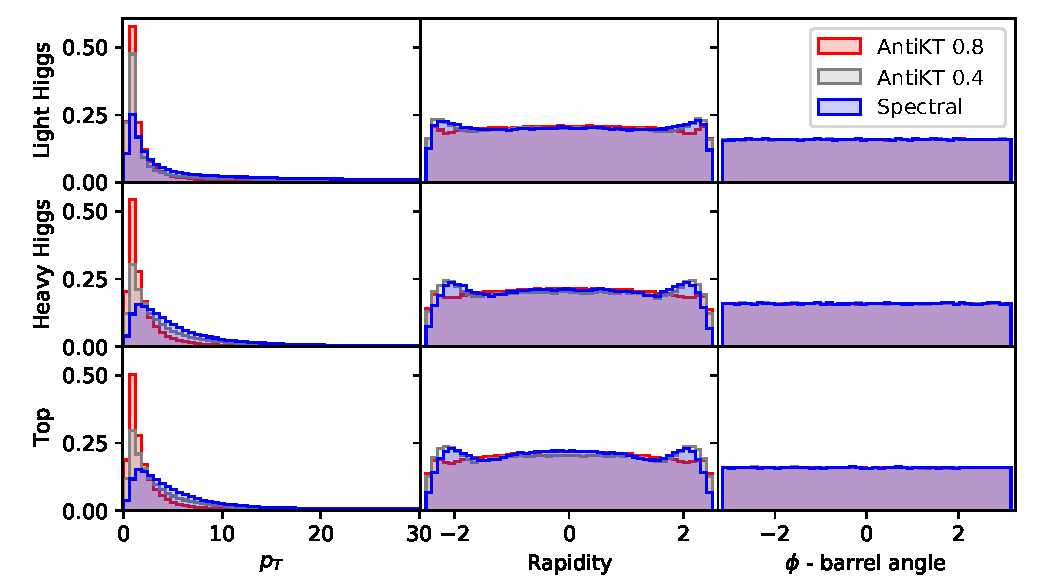
\includegraphics[width=\textwidth]{graphics/kinematics}
%\end{minipage}
    %\begin{minipage}[c]{0.25\textwidth}
        \caption{Basic jet variables for each of the analysis datasets and three clustering algorithms.
            In the first column there is some noticeable differences in the transverse momentum.
            In the second column the rapidity shows that
            the algorithms cluster jets at the edge of the barrel slightly differently.
            In the third column the barrel angle show no noticeable changes.
        }\label{fig:kinematics}
%\end{minipage}
\end{center}
\end{figure}

\subsection{IR safety}
Shape variables (see the QCD section of Ref.~\cite{Altarelli:116932} for a useful review), such as jet mass, thrust, sphericity and oblataness,  are sensitive to IR divergences.
For each configuration of the clustering algorithm we expect an IR safe algorithm to present a stable transition
in a shape variable from the LO to NLO datasets, as significant
changes in the spectra would indicate sensitivity to soft and collinear radiation.
The clustering and evaluation here is done using the \underbar{3-jets} dataset, as described in Sec.~\ref{sec:particle_data}.
Shape variables are calculated from the total momentum of the 4 jets with highest \(p_T\) in each event.
This comparison is made in Fig.~\ref{fig:IRC_singles2}.
It can be seen in this figure that little difference exists between \genkt{} and \spectral{} clustering, so as to reinforce that they are both IR safe.
{\textcolor{red}{What data set has been used here? Also, it would be woth to discuss why the distributions are so different for the case of the Mass variable. Finally, is the latter just the invariant mass formed by all tracks/particles in each jet?}\textcolor{blue}{H. I have now specifed the dataset and the choice of momentum vectors in each event. I also changed the parameters of genkt/spectral used so that they minimc each other. It just wanted a diferent parameter choice.}}

\begin{figure}[htp]
    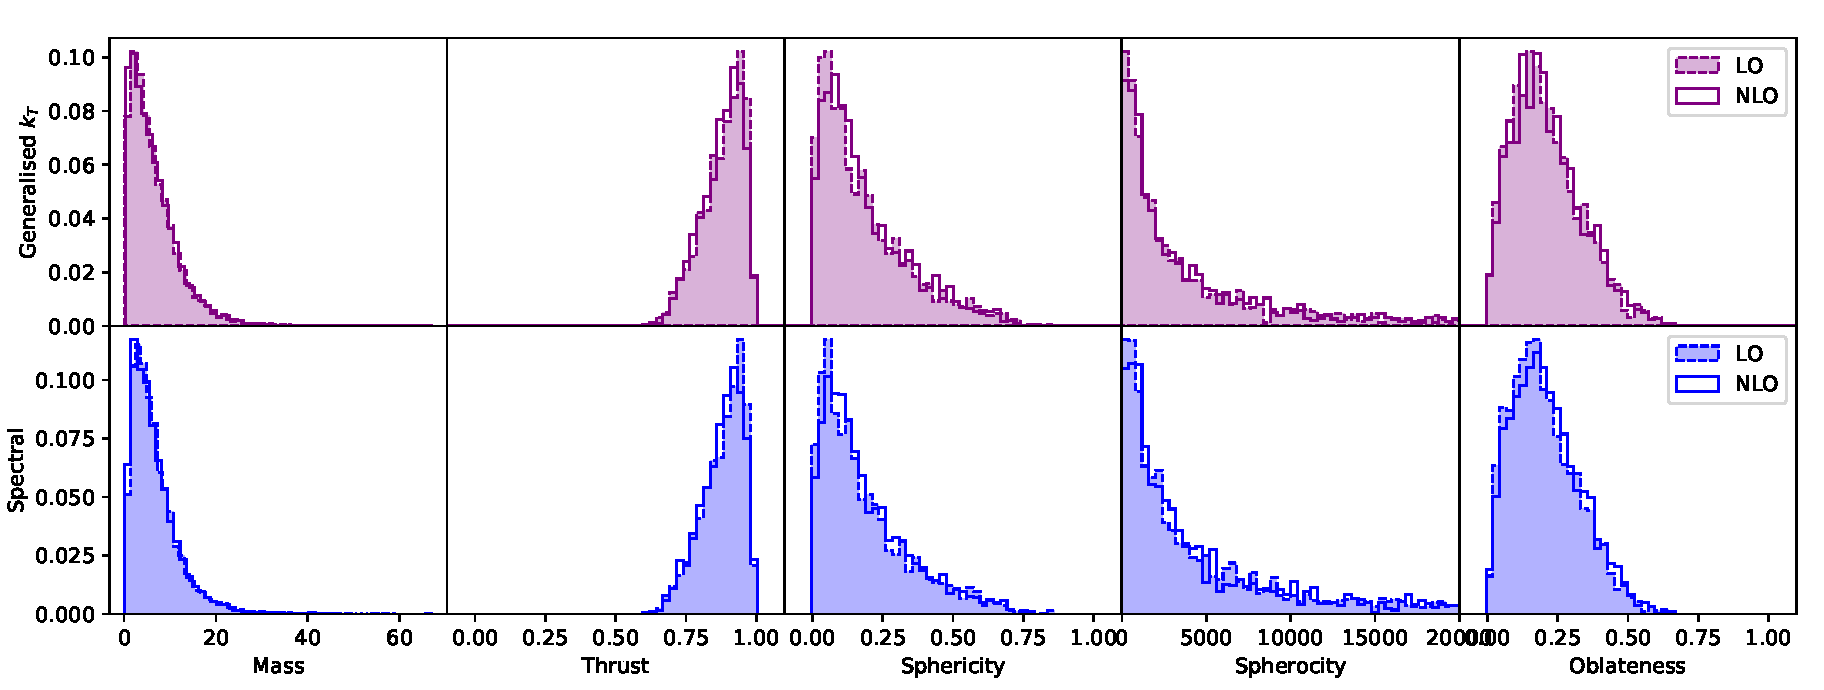
\includegraphics[width=\textwidth]{graphics/array_of_variables2_filled}
    \caption{Spectra for jet properties created with LO and NLO datasets.
             The \(4\) jets with highest \(p_T\) from each event are used in aggregate as an average to 
             form these plots.
             The columns from left to right are: the jet mass, 
             thrust, sphericity and oblateness.
             Algorithms where configured (i.e., settings of \stoppingdeltar{})
             to give sensible results on
             this dataset, therefore distributions may not represent worst case scenarios.
             %Looking at these graphs it is not immediately clear that the \genkt{}
             %algorithm is IR safe and the Iterative Cone algorithm is unsafe, 
         %much less what the status of Spectral clustering is.
         }\label{fig:IRC_singles2}
%    \begin{minipage}[c]{0.47\textwidth}
%        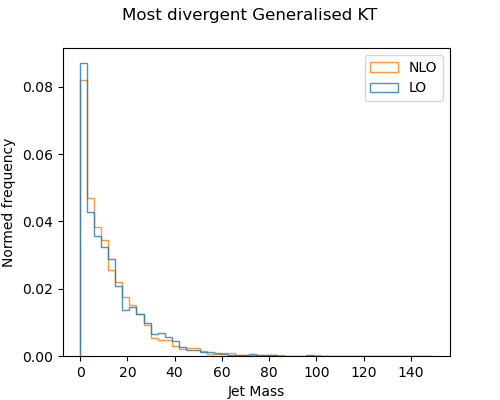
\includegraphics[width=\textwidth]{graphics/worst_antikt_histOnly.png}
         %        \caption{The jet mass spectra of the \genkt{} algorithms that
%                 differed the most between LO and NLO datasets.
%                 This algorithm had a \(p_T\) exponent of \(1.\),
%                 (so the form of the \(p_T\) factor is between Cambridge-Aachen and KT),
%                 it used taxi-cab distances in physical space
%                 and \(\stoppingdeltar{} = 1.5\).
%                 Little divergence can be seen.
%        }
%    \end{minipage}\hfill
%    \begin{minipage}[c]{0.45\textwidth}
%        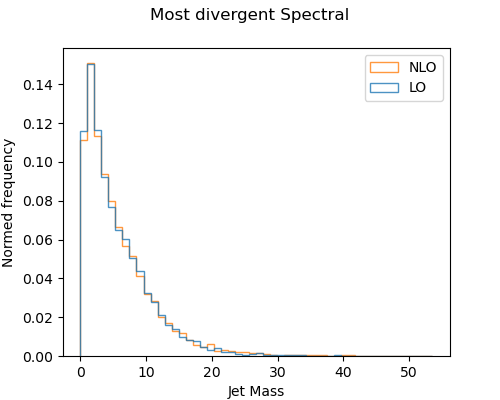
\includegraphics[width=\textwidth]{graphics/worst_spectral_histOnly.png}
%        \caption{The jet mass spectra of the Spectral algorithms that
%                 differed the most between LO and NLO datasets.
%                 This algorithm calculated affinities as
%                 \(a_{i,j} = \text{exp}\left((\delta \phi_{i, j}^2 + \delta y_{i, j}^2)/0.3\right)\).
%                 The Laplacian is symmetric and 
%                 as many eigenvector as can be found are used which are
%                 normalised as \(x_{i,\text{normed}} = x_i/\lambda_i^{1.8}\).
%                 There is no use of \(p_T\) and \(\stoppingdeltar{} = 1.3\).
%                 Little divergence can be seen.
%        }\label{fig:spectralircexample}
%    \end{minipage}
%    \begin{minipage}[c]{0.48\textwidth}
%        \includegraphics[width=\textwidth]{graphics/worst_iterativecone_histonly.png}
%        \caption{The jet mass spectra of the Iterative Cone algorithms that
%                 differed the most between LO and NLO datasets.
%                 This algorithm had a \(p_T\) exponent of \(1.\),
%                 (so the form of the \(p_T\) factor is between Cambridge-Aachen and KT),
%                 it used taxi-cab distances in physical space
%                 and \(\stoppingdeltar{} = 0.34\).
%                 Some divergence is seen, particularly at low mass.
%        }\label{fig:iterconeircexample}
%    \end{minipage}
\end{figure}    

%
%\begin{figure}[htp]
%    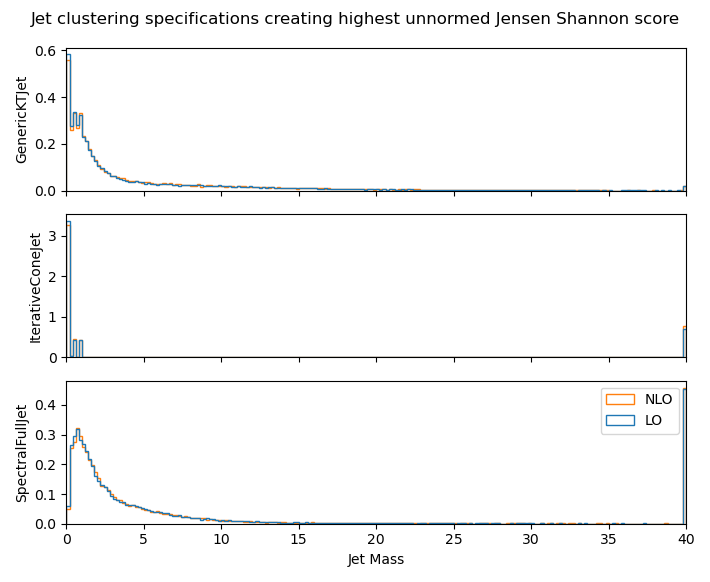
\includegraphics[width=1.\textwidth]{graphics/same_bin_size_worst_all_jets.png}
%    \caption{Same plots as previous, but with the same x-axis.
%        Last bin is overflow bin.
%    }
%\end{figure}    
%
However, this method of establishing IR safety only looks at one hyperparameter configuration and could be accused of cherry-picking.
As described in section~\ref{sec:IRmethod}, this can be systematically compared for many hyperparameter configurations by calculating a Jensen-Shannon
score for each LO and NLO pair of jet mass spectra.
If the Jensen-Shannon metric is low, then the two distributions are similar and appear IR safe.
To further clarify the result we include an algorithm known to be IR unsafe, the \itercone{} algorithm.
The spectral method produces Jensen-Shannon scores very similar to \genkt{} methods. Only the iterative cone one produces high Jensen-Shannon scores thus indicating significant changes between the LO and NLO spectra.
This can be seen in Fig.~\ref{fig:unnormedJS}. {\textcolor{red}{Is this plot done only using the Mass variable of the previous figure? If so, why this choice instead of, e.g., thrust, sphericity, oblataness or others?}\textcolor{blue}{H. fixed}}

\begin{figure}[htp]
    \begin{minipage}[c]{0.5\textwidth}
        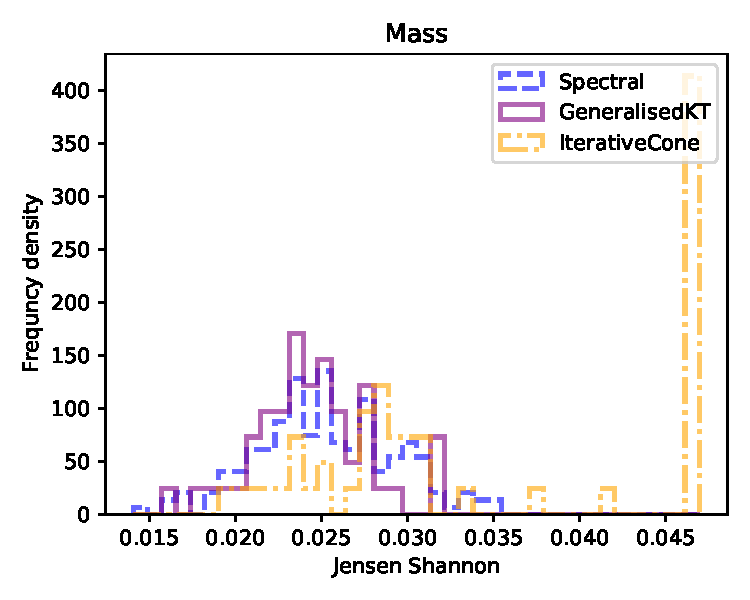
\includegraphics[width=1.\textwidth]{graphics/js_scores/Mass}
    \end{minipage}\hfill
    \begin{minipage}[c]{0.5\textwidth}
        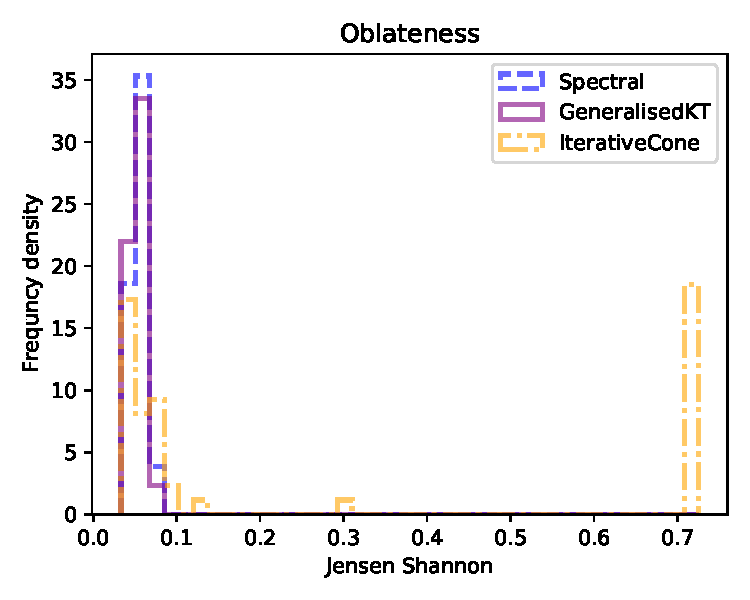
\includegraphics[width=1.\textwidth]{graphics/js_scores/oblateness}
    \end{minipage}
    \begin{minipage}[c]{0.5\textwidth}
        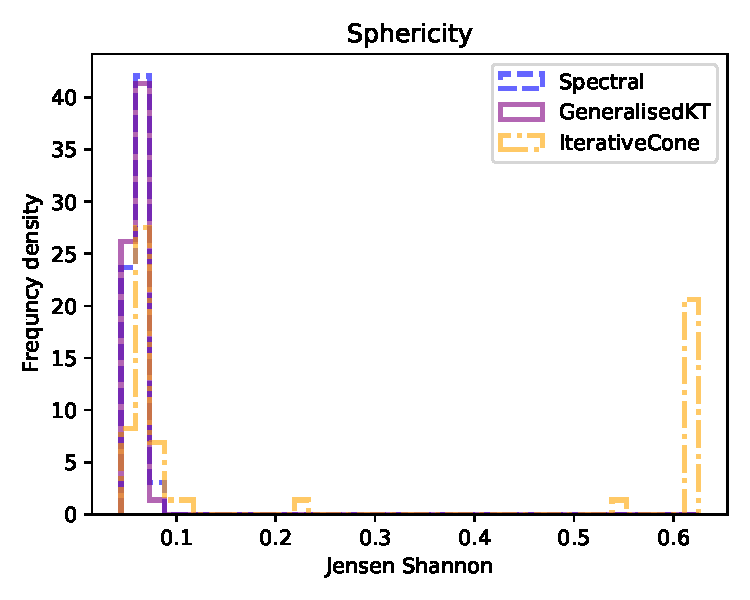
\includegraphics[width=1.\textwidth]{graphics/js_scores/sphericity}
    \end{minipage}\hfill
    \begin{minipage}[c]{0.5\textwidth}
        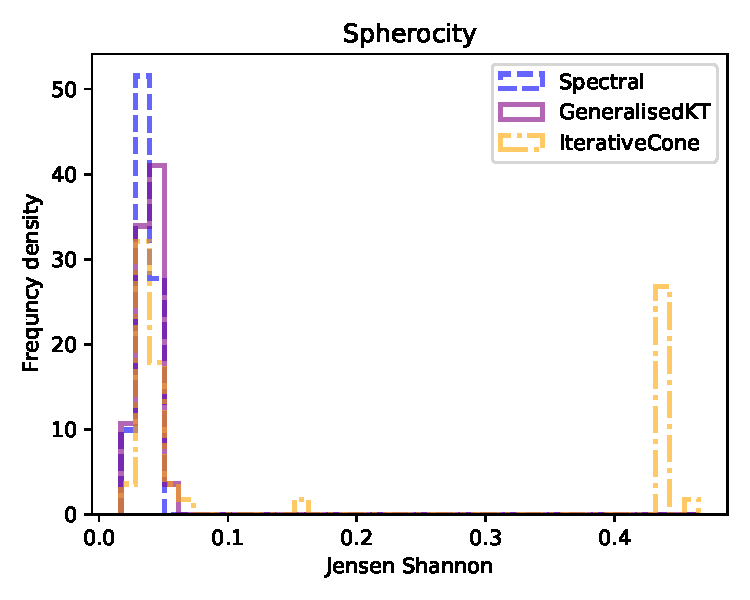
\includegraphics[width=1.\textwidth]{graphics/js_scores/spherocity}
    \end{minipage}
    \begin{minipage}[c]{0.5\textwidth}
        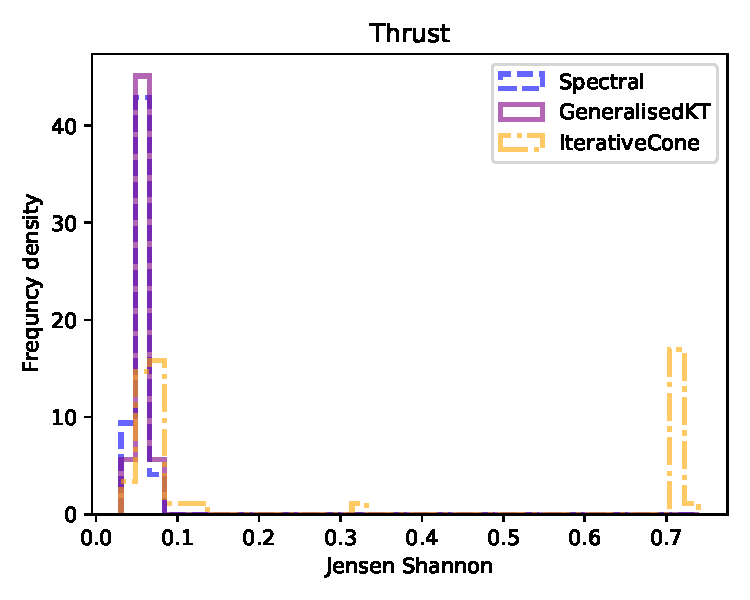
\includegraphics[width=1.\textwidth]{graphics/js_scores/thrust}
    \end{minipage}\hfill
    \begin{minipage}[c]{0.5\textwidth}
    \caption{
        Histograms evaluating IR safety from each jet shape variable.
        Each count is a  Jensen-Shannon score between a probability density of the
        jet shape variable from LO and NLO data.
        Counts at low values indicate insensitivity to IR differences between the LO and NLO data,
        thus IR safety.
     }\label{fig:unnormedJS}
    \end{minipage}
\end{figure}    

%This comparison is slightly complicated by the fact that we must use a completely different set of events,
%so if a clustering algorithm tends to produce more noisy mass spectra (on varied events), this
% will increase the gap between the LO and NLO datasets even if no IR sensitivity is present.
%Again, as described in section~\ref{sec:IRmethod}, the influence of this noise can be investigated.
%This can be seen in Fig.~\ref{fig:JensenShannon}. Here, 
%the subsampled Jensen-Shannon score is shown, again,  between a probability density of jet mass from LO and
%        NLO data, as described in section~\ref{sec:IRmethod}. Like in the previous figure, spectral clustering produces Jensen-Shannon scores similar to the \genkt{} approach. Likewise, only theiIterative cone produces high Jensen-Shannon scores, thus indicating significant changes
%        between the LO and NLO spectra. Being the results in  Figs.~\ref{fig:unnormedJS} and \ref{fig:JensenShannon} consistent with each other, this indicates  that the volume of data used to produce these
%        was sufficient to mitigate the effects of noise.

From  the last two figures it is clear that \spectral{} clustering  is IR safe, at least, as much as \genkt{} algorithms are.
This contrasts with the \itercone{} algorithm, for which the jet mass spectra at LO and NLO 
differ significantly for many configurations.
This is not unexpected, as the inputs to the \spectral{} clustering algorithm 
are the same as for the Cambridge-Aachen one, 
which is itself IR safe, and the iterative cone has been  proved to produce kinematic configurations which are IR unsafe \cite{Salam:2007xv} {\textcolor{red}{Please refer to some paper illustrating this (by Salam, Seymour, etc.)} \textcolor{blue}{H. done}} .
However, it is crucial to have such a verification in data, as we have done.

%\begin{figure}[htp]
%    \begin{minipage}[c]{0.6\textwidth}
%    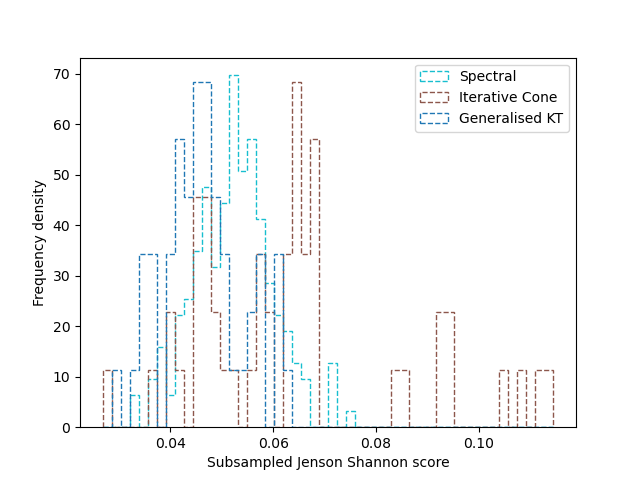
\includegraphics[width=1.\textwidth]{graphics/JensenShannon.png}
%    \end{minipage}\hfill
%    \begin{minipage}[c]{0.35\textwidth}
%    \caption{Same as Fig.~\ref{fig:unnormedJS} for the subsampled Jensen-Shannon score.
%    }\label{fig:JensenShannon}
%    \end{minipage}
%\end{figure}    

\subsection{Mass peak reconstruction}
In this section, the \antikt{} algorithm setups with jet radius \(\ktstoppingdeltar{} = 0.4\) and \(\ktstoppingdeltar{} = 0.8\)
are compared to the \spectral{} algorithm specified in section~\ref{sec:spectralmethodparam}.
The jets are tagged using MC truth.
Each of the \bthing{quarks} created by a signal particle (either a Higgs boson or a top (anti)quark)
tag the closest jet (by using the distance metric \(\sqrt{(y_\text{quark tag} - y_\text{jet})^2 + (\phi_\text{quark tag} - \phi_\text{jet})^2}\)
{\textcolor{red}{Do you really mean rapidity here or pseudorapidity? This needs to be clarified throughout as the two are not the same for massive objects} \textcolor{blue}{H. it is always rapidity, pesudorapidity is never used in this work, is Eqn~\ref{eqn:rapidity} alright?}})
provided that the separation between the jet and the quark is no greater than \(0.8\) according to the distance metric {\textcolor{red}{The sentence is unclear} \textcolor{blue}{improved?}}.
In the case of a \(W^\pm\) decay, whatever quarks decay from the \(W^\pm\), which may be light quarks or \bthing{quarks}, are used to tag jets in the same way.
From this point on, only jets tagged this way are considered {\textcolor{red}{What about light jets from $W^\pm$ decays?} \textcolor{blue}{Good point. Fixed.}}.


Firstly, jet multiplicities, that is number of reconstructed jets found per event, are given for both anti-$k_T$ and spectral clustering algorithms.
These can be seen for the first three datasets described in section~\ref{sec:particle_data} in Fig.~\ref{fig:multiplicity}. Herein, it
 is seen that \spectral{} clustering produces the best multiplicity (i.e., most events where 4 jets are found) for light Higgs events while for 
         the heavy Higgs and top MC samples  
        it creates a multiplicity closer to that of \antikt{} with \(\ktstoppingdeltar{} = 0.4\) 
        than \(\ktstoppingdeltar{} = 0.8\), the first of these being the best performer of the two. As a result of this study, we remark upon the adaptability of spectral clustering to the different final states without requiring adjusting its parameters, unlike the anti-$k_T$ one. The latter may seem to indicate that 0.4 is the best choice for all datasets, but this is in tension with the fact that different masses from different datasets do require the  anti-$k_T$ algorithm to be adjusted, as we shall now see. 



\begin{figure}[htp]
    \begin{center}
        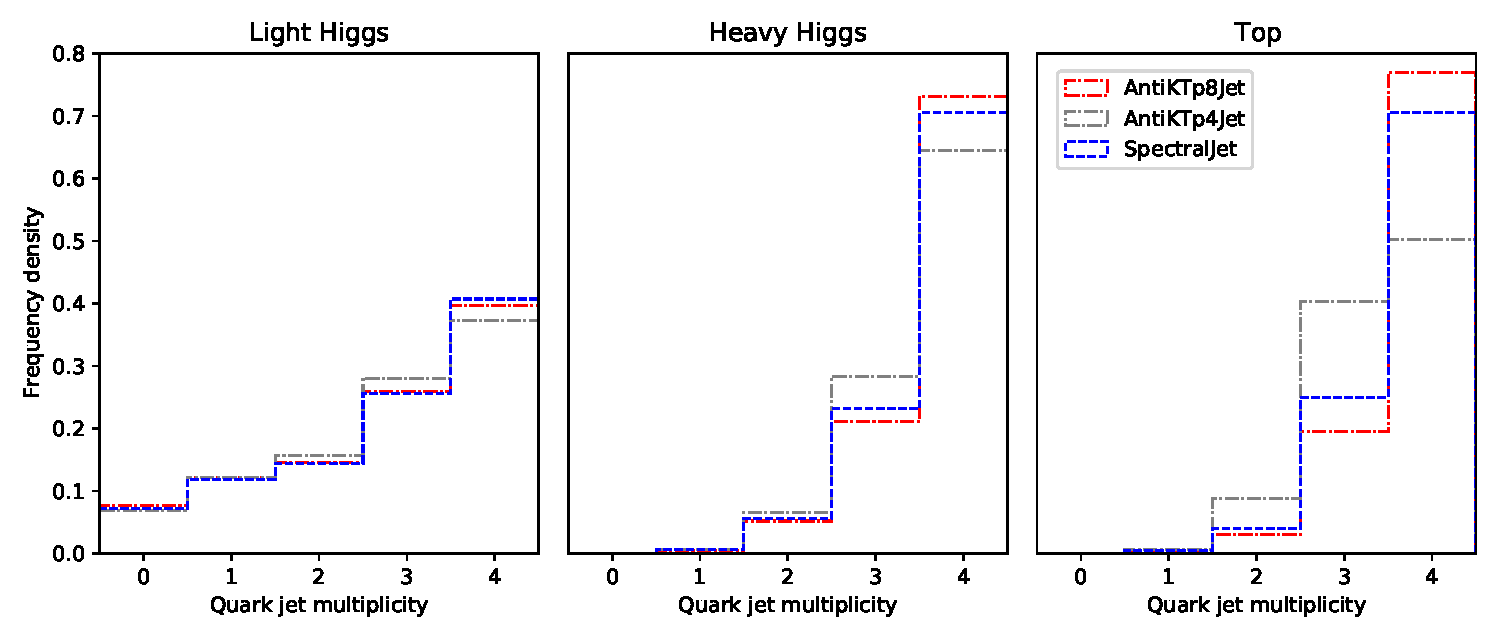
\includegraphics[width=1.0\textwidth]{graphics/multiplicity/multiplicity}
    \end{center}
    \caption{Jet multiplicities for the anti-$k_T$ (for two jet radius choices) and \spectral{} clustering algorithms on the light Higgs, heavy Higgs and top MC 
 samples. For all such datasets, the hard scattering produces  4 partons in the final  state, so maximising a multiplicity of 4 jets indicates good performance.   
    }\label{fig:multiplicity}
\end{figure}    



%As the data is simulated, it is possible to compare the performance of clustering algorithms to Monte Carlo truth.
%Each Higgs cascade event contains 4 \bthing{quarks} and for each of them it is possible to identify the particle into which they decayed, as a subset of the particles in the final state.
%Henceforth the detectable decay products of the \bthing{quark} will be called the descendants of the \bthing{quark}.
%For two reasons it is not possible for this clustering algorithm to gather all the descendants
%of each \bthing{quark} into one jet:
%firstly, not all the descendants make the \(p_T\) and \(\eta\) cuts, so some are discarded before clustering;
%secondly, the descendants of the \bthing{quarks} in an event are not mutually exclusive, due to interactions during hadronisation the quarks share descendants, and our clustering algorithm does produce exclusive clusters.
%
%Combining these factors with the \(p_T\) cuts, almost \(2/3\) of the objects could be reconstructed in theory.

%Knowing the parts of the final state that are descended from each \bthing{quark} creates a clear
%allocation of jets to quarks.
%For each quark, the jet that contains the greatest mass in descendent particles is tagged to represent that quark.

Mass peaks are constructed from the reconstructed jets as well as, for the top sample only, from the lepton and neutrino.
Again, the \antikt{} results  with \(\stoppingdeltar{}_{k_T} = 0.4\) and \(0.8\) are given for comparison.
In Fig.~\ref{fig:best_correct_h_allocation} three selections are plotted. Firstly, we show events where all 4 $b$-jets  
are plotted as total invariant mass of the event, thus reconstructing the mass of the SM Higgs boson.
Each event also contains two light Higgs states, though. These are differentiated by the mass of the particles (generating them) that pass the particle cuts,
as follows. The light Higgs boson reconstructed from the 2 $b$i-jet system with more mass visible to the detector is called the ``Light Higgs with stronger signal''
while the one reconstructed  with less mass visible in the detector is called the ``Light Higgs with weaker signal'' {\textcolor{red}{I do not really like this wording, I would suggest instead ``Most massive light Higgs'' and ``Lest massive light Higgs''} \textcolor{blue}{H., I don't think the mass of the higgs itself (the displacement offshell) has much influence on which higgs is which. It's a reflection of which higgs produces more decay products that pass the particle cuts, whcih reflect the detectors capacity to reconstruct particles according to pt and rapidity. What do you think of; ``Higgs producing stronger signal"/``Higgs producing weaker signal"?}}.
%Two jets are required to reconstruct a light Higgs.
The correct jets for each Higgs mass reconstruction are identified using MC truth,
so the correct pairings are always made. (If two such di-jet systems are not found the event is not included in the plots).
Altogether, it can be seen that spectral clustering forms the sharpest peaks and such peaks are all very close to the correct mass. In fact, its performance
is comparable to that of anti-$k_T$ with jet radius 0.8 and is clearly better than the 0.4 option. 


\begin{figure}[htp]
    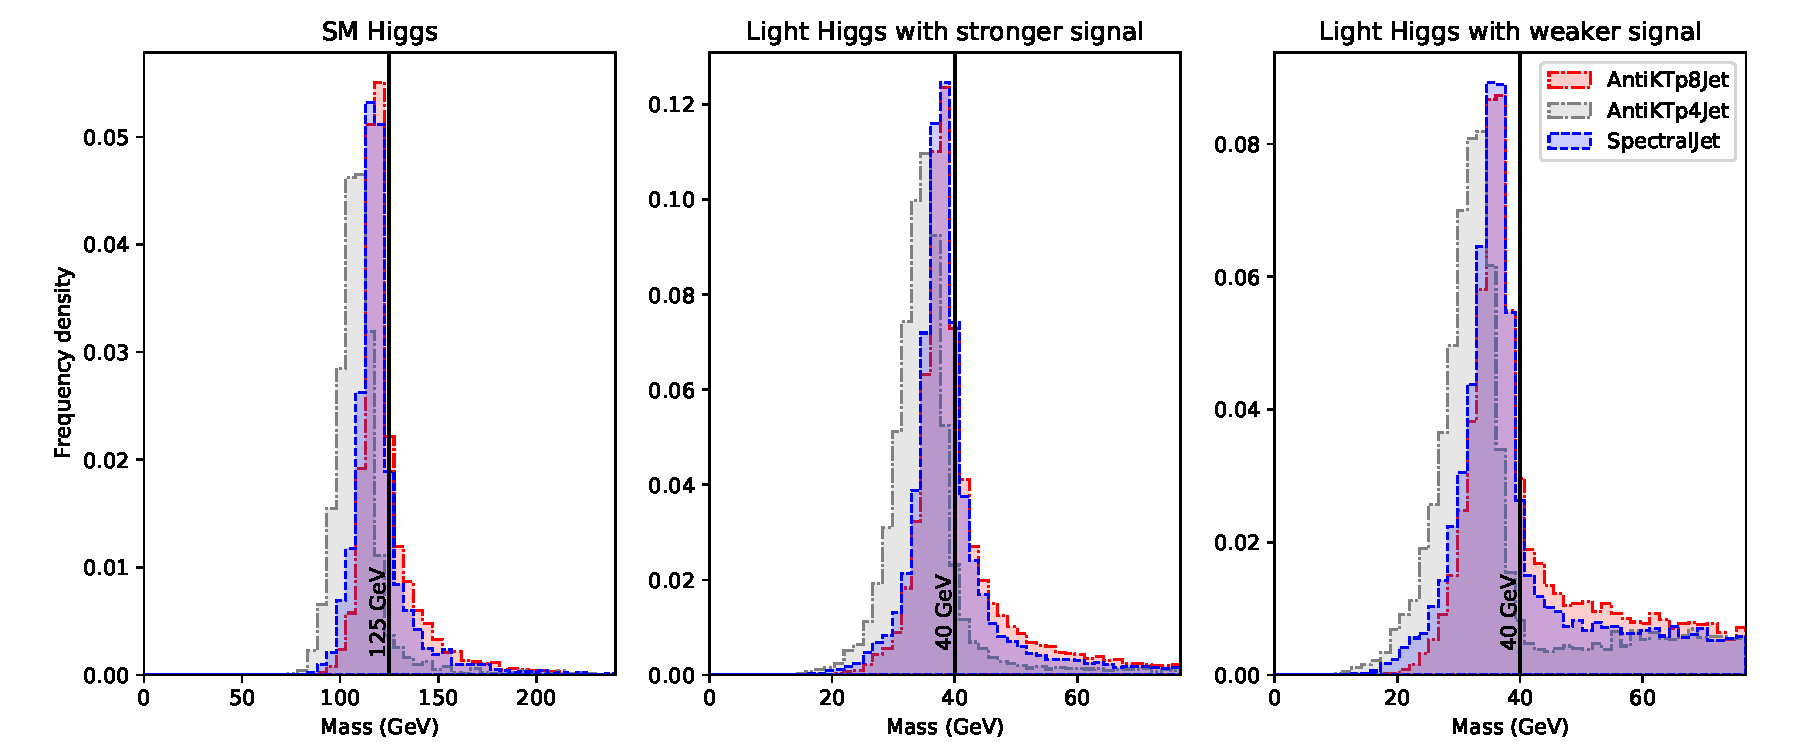
\includegraphics[width=1.\textwidth]{graphics/mass_peaks/light_long_correct_lines}
    \caption{Three mass selections are plotted for the light Higgs dataset. From left to right we show: the invariant mass of the 4 $b$-jet system, of the 2 $b$-jet system with heaviest invariant mass and of the 2 $b$-jet system with lightest invariant mass (as defined in the text).   Three jet clustering combinations are plotted as detailed in the legend.
        The spectral clustering algorithm is consistently the best performer in terms of the narrowest peaks being reconstructed and comparable to \antikt{} with \(\ktstoppingdeltar{} = 0.8\) in terms of its shift from the true Higgs mass values, with \antikt{} with \(\ktstoppingdeltar{} = 0.4\) always being the outlier. 
{\textcolor{red}{Higgs should be capitalised as Higgs in the top titles, though, see my remark in the body for the actual names} \textcolor{blue}{H. done}}
    }\label{fig:best_correct_h_allocation}
\end{figure}    

In 
Fig.~\ref{fig:heavy_correct_mass_peaks} the exercise is repeated for the heavy Higgs dataset.
All the parameters of \spectral{} clustering are the same as in the light Higgs MC sample yet we note that 
its performance is still excellent, with very sharp peaks at the correct masses, although the three clustering algorithms are overall much closer in performance.
However, recall that, in Fig.~\ref{fig:multiplicity},
it was seen that spectral clustering achieved better multiplicity than \antikt{} with \(\ktstoppingdeltar{} = 0.8\) on this dataset. Furthermore, 
while the multiplicity of \antikt{} with \(\ktstoppingdeltar{} = 0.4\) is a little better, the location of all Higgs mass peaks for anti-$k_T$ with 
\(\ktstoppingdeltar = 0.4\) is slightly worse. So, we are again driven to conclude that spectral clustering is probably the best performer overall with the added benefit of not requiring any adjustment of its parameters to achieve it. 

\begin{figure}[htp]
    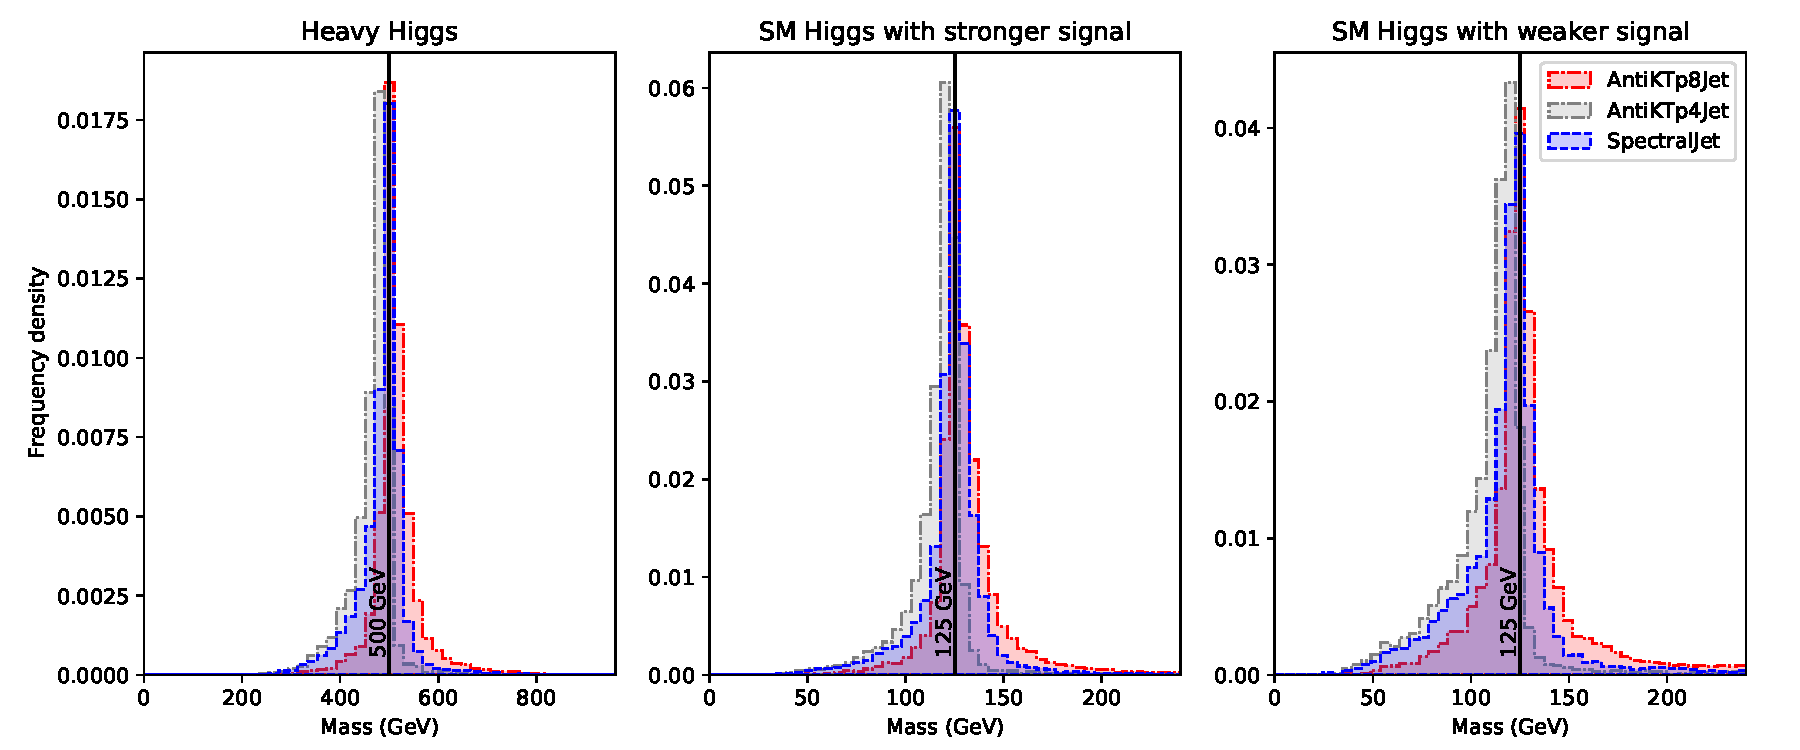
\includegraphics[width=1.\textwidth]{graphics/mass_peaks/heavy_long_correct_lines}
    \caption{Same as Fig.~\ref{fig:best_correct_h_allocation} for the heavy Higgs dataset. Here, the performance of the spectral clustering and anti-$k_T$ (with both 0.4 and 0.8 as jet radiuses) clustering is much closer to each other. 
}\label{fig:heavy_correct_mass_peaks}
\end{figure}    


\begin{figure}[htp]
    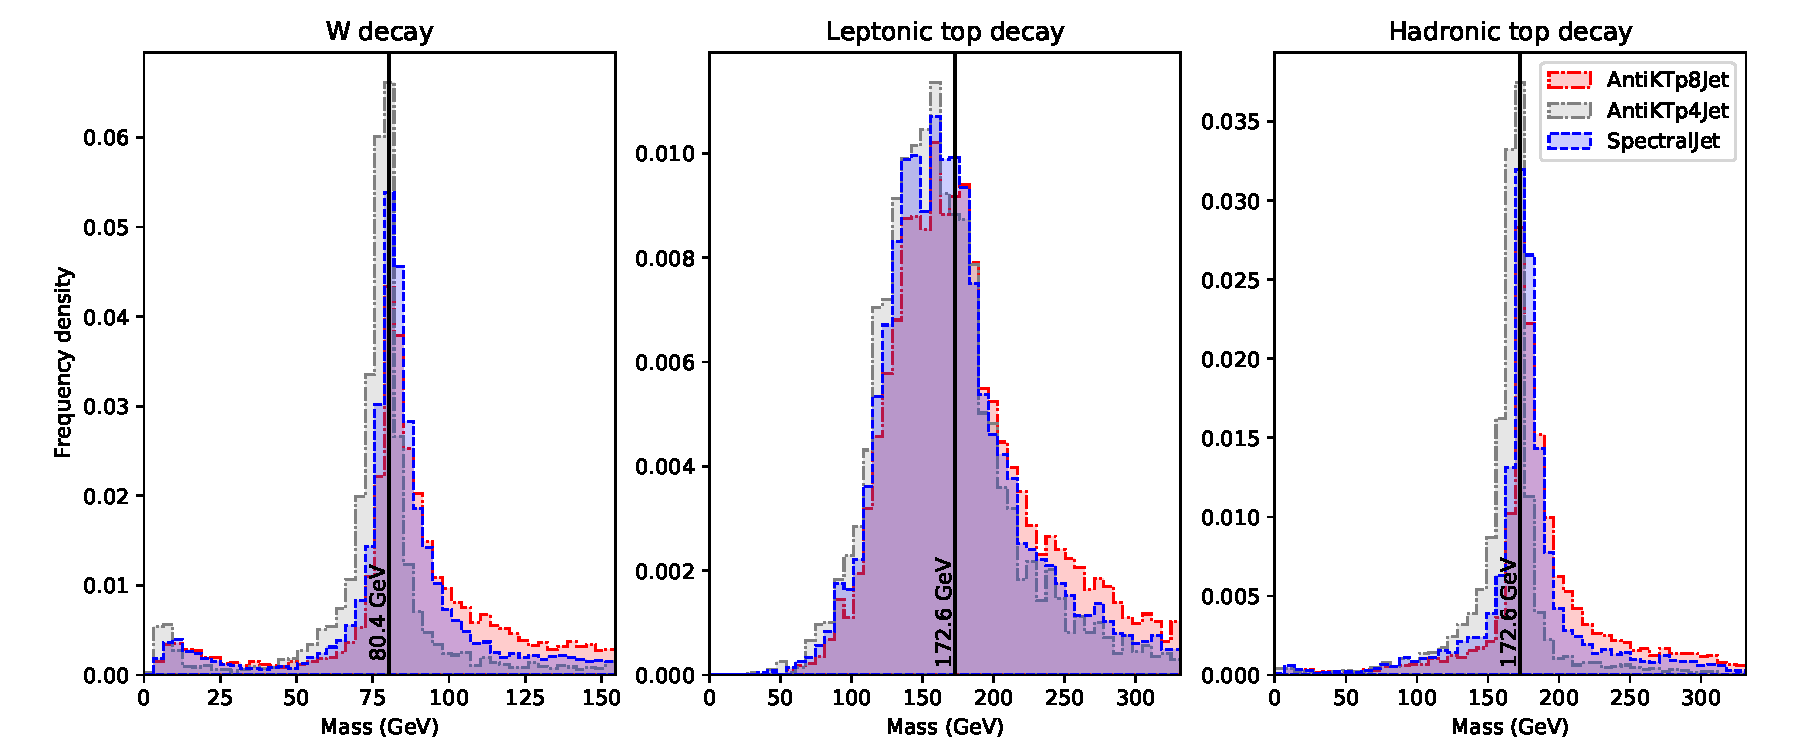
\includegraphics[width=1.\textwidth]{graphics/mass_peaks/top_long_correct_lines}
    \caption{Three mass selections are plotted for the top dataset. From left to right we show: the invariant mass of the light jet system, of the reconstructed leptonic $W^\pm$ (as  described in the text) combined with a $b$-jet and of the hadronic $W^\pm$ combined with the other $b$-jet. Three jet clustering combinations are plotted as detailed in the legend.
The spectral clustering algorithm  consistently outperforms the  anti-$k_T$ one with jet radius 0.8 and is slightly worse than the anti-$k_T$ one with jet radius 0.4, but only in tems of sharpness, not location.
    }\label{fig:top_correct_mass_peaks}
\end{figure}    

Finally, in Fig.~\ref{fig:top_correct_mass_peaks}, the $W^\pm$ and $t$ mass peaks for semileptonic $t\bar t$ decays are shown.
Three mass reconstructions are given.
Firstly, the hadronic \(W\) is reconstructed from the jets that come from the quarks it decayed to.
Correct decisions about which quarks correspond to which particle in the hard process are made by using information in the Monte Carlo,
this is to prevent any mismatching from causing additional complication in evaluating the performance of the clustering.
To tag a jet with a quark a distance measure \(\sqrt{(y_\text{quark tag} - y_\text{jet})^2 + (\phi_\text{quark tag} - \phi_\text{jet})^2}\)
is used, and if the distance from the quark to the closest jet is less than \(0.8\) that jet is tagged by that quark.
The \(W\) will always decay to a pair of quarks, but both these quarks may be captured in one jet or separate jets.
{\textcolor{red}{This sentence did not make sense at all} \textcolor{blue}{H. is this better?}}.
If either of the these quarks are too far away from the closest jet to tag it,
that is \(\sqrt{(y_\text{quark tag} - y_\text{jet})^2 + (\phi_\text{quark tag} - \phi_\text{jet})^2} > 0.8\),
then it is not associated with any jet and the hadronic \(W\) is not reconstructed.
{\textcolor{red}{This sentence did not make sense either} \textcolor{blue}{H. is this better?}}.
The mass of the hadronic top is then reconstructed in events where the hadronic \(W\) could be reconstructed and the \bthing{jet}
from the hadronic top is also found. {\textcolor{red}{By MC truth or you pick the $b$ that gives the best $m_t$? Please clarify} \textcolor{blue}{H., always MC truth, I will clarify this at the start of the passage.}}.
The leptonic top is then reconstructed in events where \bthing{jet} from the top is combined with the reconstructed $W^\pm$ which as decayed leptonically
{\textcolor{red}{By MC truth or pick the $b$ that gives the best $m_t$? Please clarify}\textcolor{blue}{H. ditto}}.
The leptonic reconstruction of the $W^\pm$ uses the momentum of the electron $p_\ell$, the missing transverse momentum $p_T^{\rm miss}$ (identified with that of the neutrino)
and the longitudinal neutrino momentum ($p_L^\nu$, which is unknown) in a quadratic equation, $(p_\ell+p_T^{\rm miss}+p_L^\nu)^2=m_W^2$, of which only the real solutions are plotted.  In this case, it can be seen that \spectral{} clustering is adapting to jets of a different radius. In fact, 
while before its behaviour had mostly resembled anti-$k_T$ with \(\ktstoppingdeltar{} = 0.8\), 
it has now moved closer to the case with \(\ktstoppingdeltar{} = 0.4\).
(Semileptonic top events would typically be processed using anti-$k_T$ with \(\ktstoppingdeltar{} = 0.4\).)
The peaks of \spectral{} clustering are not quite as narrow as those from anti-$k_T$ with \(\ktstoppingdeltar{} = 0.4\),
but they improve on \(\ktstoppingdeltar{} = 0.8\) and their  location is substantially correct.

%\begin{figure}[htp]
%    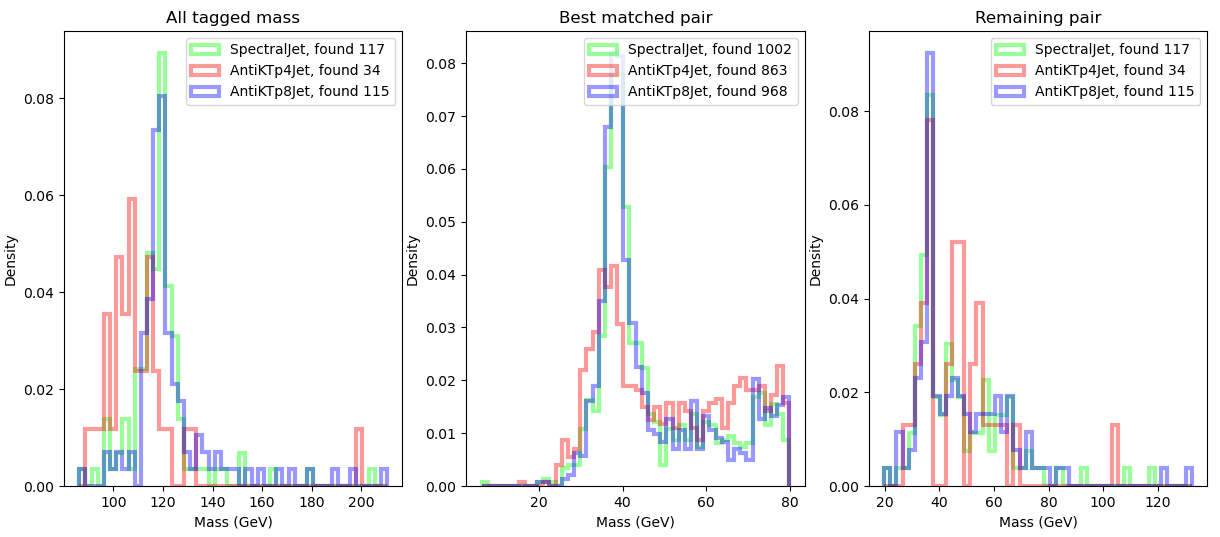
\includegraphics[width=1.\textwidth]{graphics/show2_40.png}
%    \caption{Mass peaks for the light Higgs cascade;
%    \(p^+ p^+ \rightarrow H_{125\text{GeV}} \rightarrow h_{40\text{GeV}} h_{40\text{GeV}} \rightarrow \beau \bbar \beau \bbar\).
%        Jets are required to have at least 2 particles and \(15\) GeV \(p_T\).
%        The left hand peak is the mass of all jets in events where 4 jets are reconstructed.
%        The central plot is the mass of the dijet pair closest to \(40\) GeV,
%        the right hand plot is the remaining dijet pair.
%    }
%\end{figure}    
%
%\begin{figure}[htp]
%    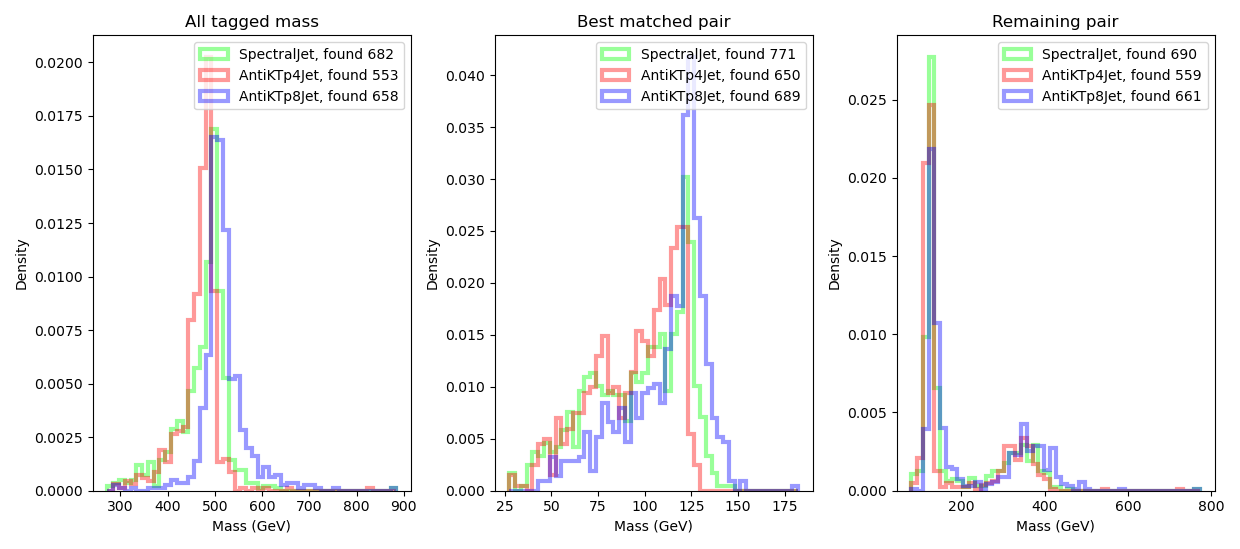
\includegraphics[width=1.\textwidth]{graphics/show2_125.png}
%    \caption{Mass peaks for the heavy Higgs cascade,
%    \(p^+ p^+ \rightarrow H_{500\text{GeV}} \rightarrow h_{120\text{GeV}} h_{120\text{GeV}} \rightarrow \beau \bbar \beau \bbar\).
%        Jets are required to have at least 2 particles and \(30\) GeV \(p_T\).
%        The left hand peak is the mass of all jets in events where 4 jets are reconstructed.
%        The central plot is the mass of the dijet pair closest to \(125\) GeV,
%        the right hand plot is the remaining dijet pair.
%    }
%\end{figure}    



%There are also some values that can be given to compare these two jets;
%\begin{enumerate}
%    \item Quality fraction~\cite{JetQuality2008}. A window on the reconstructed masses,
%        size proportional to the root of mass of the object to be reconstructed,
%        across the data. The total number of generated objects (in this dataset 2000)
%        is divided by the maximum number of reconstructed objects in the window,
%        and this is the quality width.
%        
%        \[\text{\antikt{} (\(\stoppingdeltar{} = 0.8\)) Quality Fraction} = 1.33\text{GeV}\]
%        \[\text{Spectral Quality Fraction} = 1.33\text{GeV}\]
%    \item Quality width~\cite{JetQuality2008}. A required fraction of the generated objects,
%        in this case \(0.15\) is selected.
%        The smallest mass window that can capture this fraction is determined.
%        
%        \[\text{\antikt{} (\(\stoppingdeltar{} = 0.8\)) Quality Width} = 0.00141\text{GeV}\]
%        \[\text{Spectral Quality Width} = 0.000129\text{GeV}\]
%    \item Signal mass lost. The mass of the particles descendent from the light Higgs
%        that are visible on the barrel is compared to the mass of the subset of those
%        particles that was found in the jet. The higher the number the more
%        signal particles are missing from the jet.
%        \[\text{\antikt{} (\(\stoppingdeltar{} = 0.8\)) Signal mass lost} = 1.80\text{GeV}\]
%        \[\text{Spectral Signal mass lost} = 2.17\text{GeV}\]
%    \item Background contamination. The mass of all the background objects,
%        either from the wrong Higgs or from gluons, found in jets.
%        The higher the number the more the jets are tending to include too many particles.
%        \[\text{\antikt{} (\(\stoppingdeltar{} = 0.8\)) Background contamination} = 1.92\text{GeV}\]
%        \[\text{Spectral Background contamination} = 1.56\text{GeV}\]
%\end{enumerate}
%

    \FloatBarrier
    \section{Conclusions}
Spectral clustering offers a promising new jet formation method.
It is a transparent mechanism with no black box element.
All intermediate steps are interpretable.
It satisfies the need for IRC safety and creates jets with the expected kinematics.

While it has many hyperparameters, then do not appear to be as finely tuned as those of \genkt{}.
This can be seen both in parameter scans, and its adaptability to various datasets.

The adaptability between datasets is remarkable,
a \spectral{} parameter choice tuned on a light higgs cascade
gave excellent performance on both a heavy higgs cascade and a top decay.
On the light higgs cascade \spectral{} gives the correct mass peak,
a narrow mass peak and the highest multiplicity.
This would not be surprising as it was tuned for that dataset.
On the heavy higgs dataset only \antikt{} \(\ktstoppingdeltar{} = 0.8\) 
and \spectral{} give correct mass peaks, and \spectral{} offers considerably higher multiplicities.
This demonstrates that the performance is not dependent on fine tuning and the algorithm is adaptable.

Finally, \spectral{} was applied to a dataset for which the ideal jet radius differed.
Its equivalent parameter \(\sigma_v\) was not allowed to vary to account for this,
instead it was applied again with no parameter changes.
The algorithm again proved to be adaptable and modified its behaviour to follow that of \(\ktstoppingdeltar{} = 0.4\)
without interference.

This is a novel and promising approach to jet formation. 
Initial development already demonstrates flexibility and excellent performance.


    \FloatBarrier
    \FloatBarrier
\section{Jet Classification}\label{sec:jetclasification}
Jet classification attempts to identify the signal jets,
commonly those containing quark descendants,
and further identify the flavour of the quark.
Typically this begins with a process known as expert feature selection \cite{CMS_CSVDeepCSV13TeV, Schramm:2291608}.
Expert feature selection, also sometimes called handcrafted features, is the process of defining variables on jets of tracks inspired by physics knowledge.
These features hope to provide good discriminating power between different types of jet.
The most successful example of this is perhaps the n-subjettiness, others include jet \(p_T\) and jet area.

Expert features are often criticised for requiring redesigning for each problem, and for potential information loss \cite{cheng_recursive_2018, radovic_machine_2018}.
Others have come out in favour of expert feature selection, however. In \cite{Lin_boostingbbH2018} expert feature selection is compared to a neural network approach that retains all information and the author reports that ``the most power is gained from a Neural Network, although we have shown that a large fraction of this information can be obtained through simple observables.".

There are a number of systematic ways for generating features akin to expert features for jets;
The Lund Plane~\cite{Dreyer_LundPlane2018} generates new features in a way that is easy to visualise and can create a linear sequence for a jet.
This involves plotting tracks that split from the central track on the relative \(p_T\) - relative angle plane to generate density maps.
Cuts can be used to impose IR and collinear safety.
This feature should lend itself to visualisation of trends.
Another such system has been dubbed energy flow polynomials~ \cite{Komiske_flowPolynomials2018}.
Energy flow polynomials (EFP) constitute a complete basis for all IR collinear safe features for a jet.
The author of \cite{Komiske_flowPolynomials2018} emphasises that commonly chosen expert features are found by combing only a few terms in the EFP.

Machine learning tools are capable of fitting highly non-linear signals,
so it might be possible to use them to bypass expert feature selection all together.

\subsection{Recursive Neural Tensor Networks}
% pros and cons of each method considered
There are many possible forms for a neural network that classifies jets;
\begin{itemize}
    \item A feed forward Deep Neural Network (DNN). This is simple to train but requires a fixed length input.
        Obtaining a fixed length input is a challenge because the number of tracks in a jet is not fixed,
        expert features must be used, and often some form of interpolation or padding is required. 
        This doesn't make a DNN a very natural fit for the problem.
    \item A Convolutional Neural Network (CNN). This can be run on an image generated by the calorimeter output.
        It has the advantage of interpretability because the filters it developed to scan the image can be analysed and some of it's process can be estimated.
        Removing symmetries from the images, however, is difficult to achieve without distorting their physical content.
        Rotations in particular are frequently done improperly, altering the jet mass.
        Further, the images are sparse, and a CNN focuses on local correlations so cannot perform optimally on spares images.
    \item A Recurrent Neural Network (RNN). This can read in a sequence, so if we could order the tracks it would be able to used all there data.
        Finding a natural ordering for the tracks is difficult, however.
        Previously \(p_T\) has been used, the Lund Plane is certainly a natural ordering,
        but it doesn't capture all the tracks.
    \item A Recurrent Neural Tensor Network (RTRN). RTRNs follow a tree shape, being originally developed for parsing syntax trees.
        This happens to coincide exactly with the shape of a jet clustering algorithm, so we could apply them to this.
\end{itemize}
% add something about all the thoughts on zero padding
To begin with the starting point considered was DeepCSV. It is a DNN, so it's foible is a fixed length input vector.
As each input is one jet long, two types of variable are considered, variables that describe an aspect of the jet as a whole
(\(p_T\) of the jet for instance) or variables that describe an aspect of a single track (such as \(p_T\) of that track).
The first kind have a fixed length and provided all values are successfully reconstructed (which is not always true)
will require no `padding'.
Padding is the manner in which missing values are filled.
The second kind, variables per track, will not have a fixed length even if the reconstruction is perfect because the number of tracks in a jet varies.
Unless the plan is to train a separate DNN for each size of jet (which would be statistically wasteful and computationally expensive)
some form of padding will have to be chosen.

The amount of padding required for a restricted set of tracks in my dataset is shown in figure~\ref{fig:prog_unreconstructed}.
\begin{figure}
    \centering
    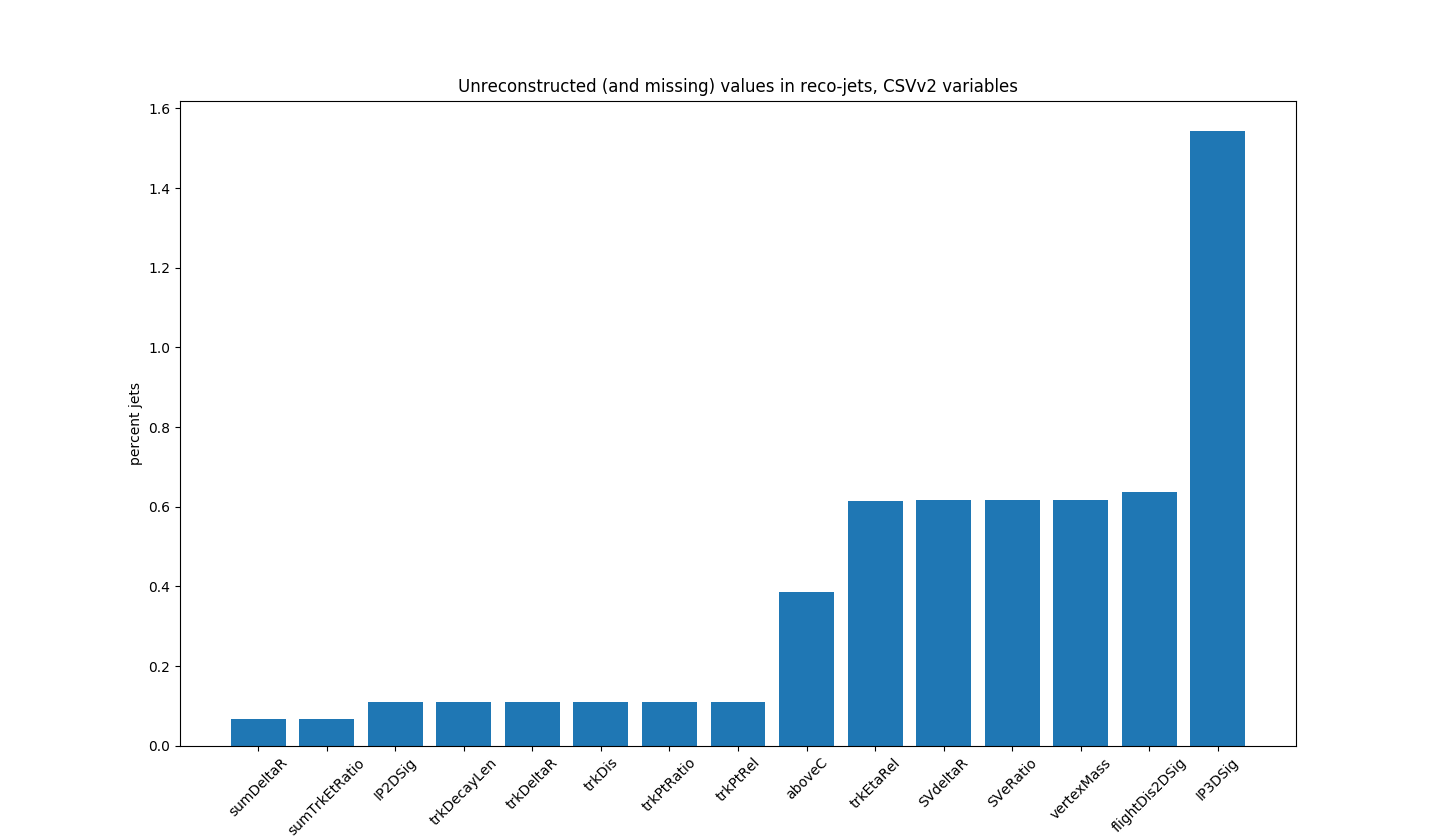
\includegraphics[width=0.8\textwidth]{images/prog_unreconstructed.png}
    \caption{Both DeepCSV and CSVv2 used zero padding to fill in values that were not available from the data. In my data sample the percentage of each variable that must be zero padded for CSVv2 is shown here.}
    \label{fig:prog_unreconstructed}
\end{figure}

The padding decision taken in~\cite{CMS_CSVDeepCSV13TeV} was called zero padding, 
but as the distributions are all centred on zero before padding this is equivalent to padding with the average value of each distribution.
Thus we can imagine that we are inserting ``average" tracks into each event until there are sufficient tracks to fill the fixed length input.
This make very little physical sense; the momentum of the additional tracks will contradict the momentum of the jet, and the angle of the tracks
will have no relation to the angle of the jet at all.

This was deemed to be an undesirable approach, so new methods that didn't require fixed length input were considered.

\subsubsection{Picture from the Monte Carlo}

In order to better envision a good neural network some time was spend graphing the behaviour of a selection of Monte Carlo showers and their jets.
A shower from a heavy Higgs decay can be seen in figure~\ref{fig:prog_bjetShower}.
Here showers are considered to start with the particles that leave the hard event, and any child of the proton beam besides the hard interaction.
These are dubbed originating particles. 
Any descendant of an originating particle is in the originating particle's shower.
Due to the requirements of colour confinement, if any originating particle is colour charged it must share descendants with another shower
so that the final descendants are colour neutral.
This happens in hadronisation.

\begin{sidewaysfigure}
    \centering
    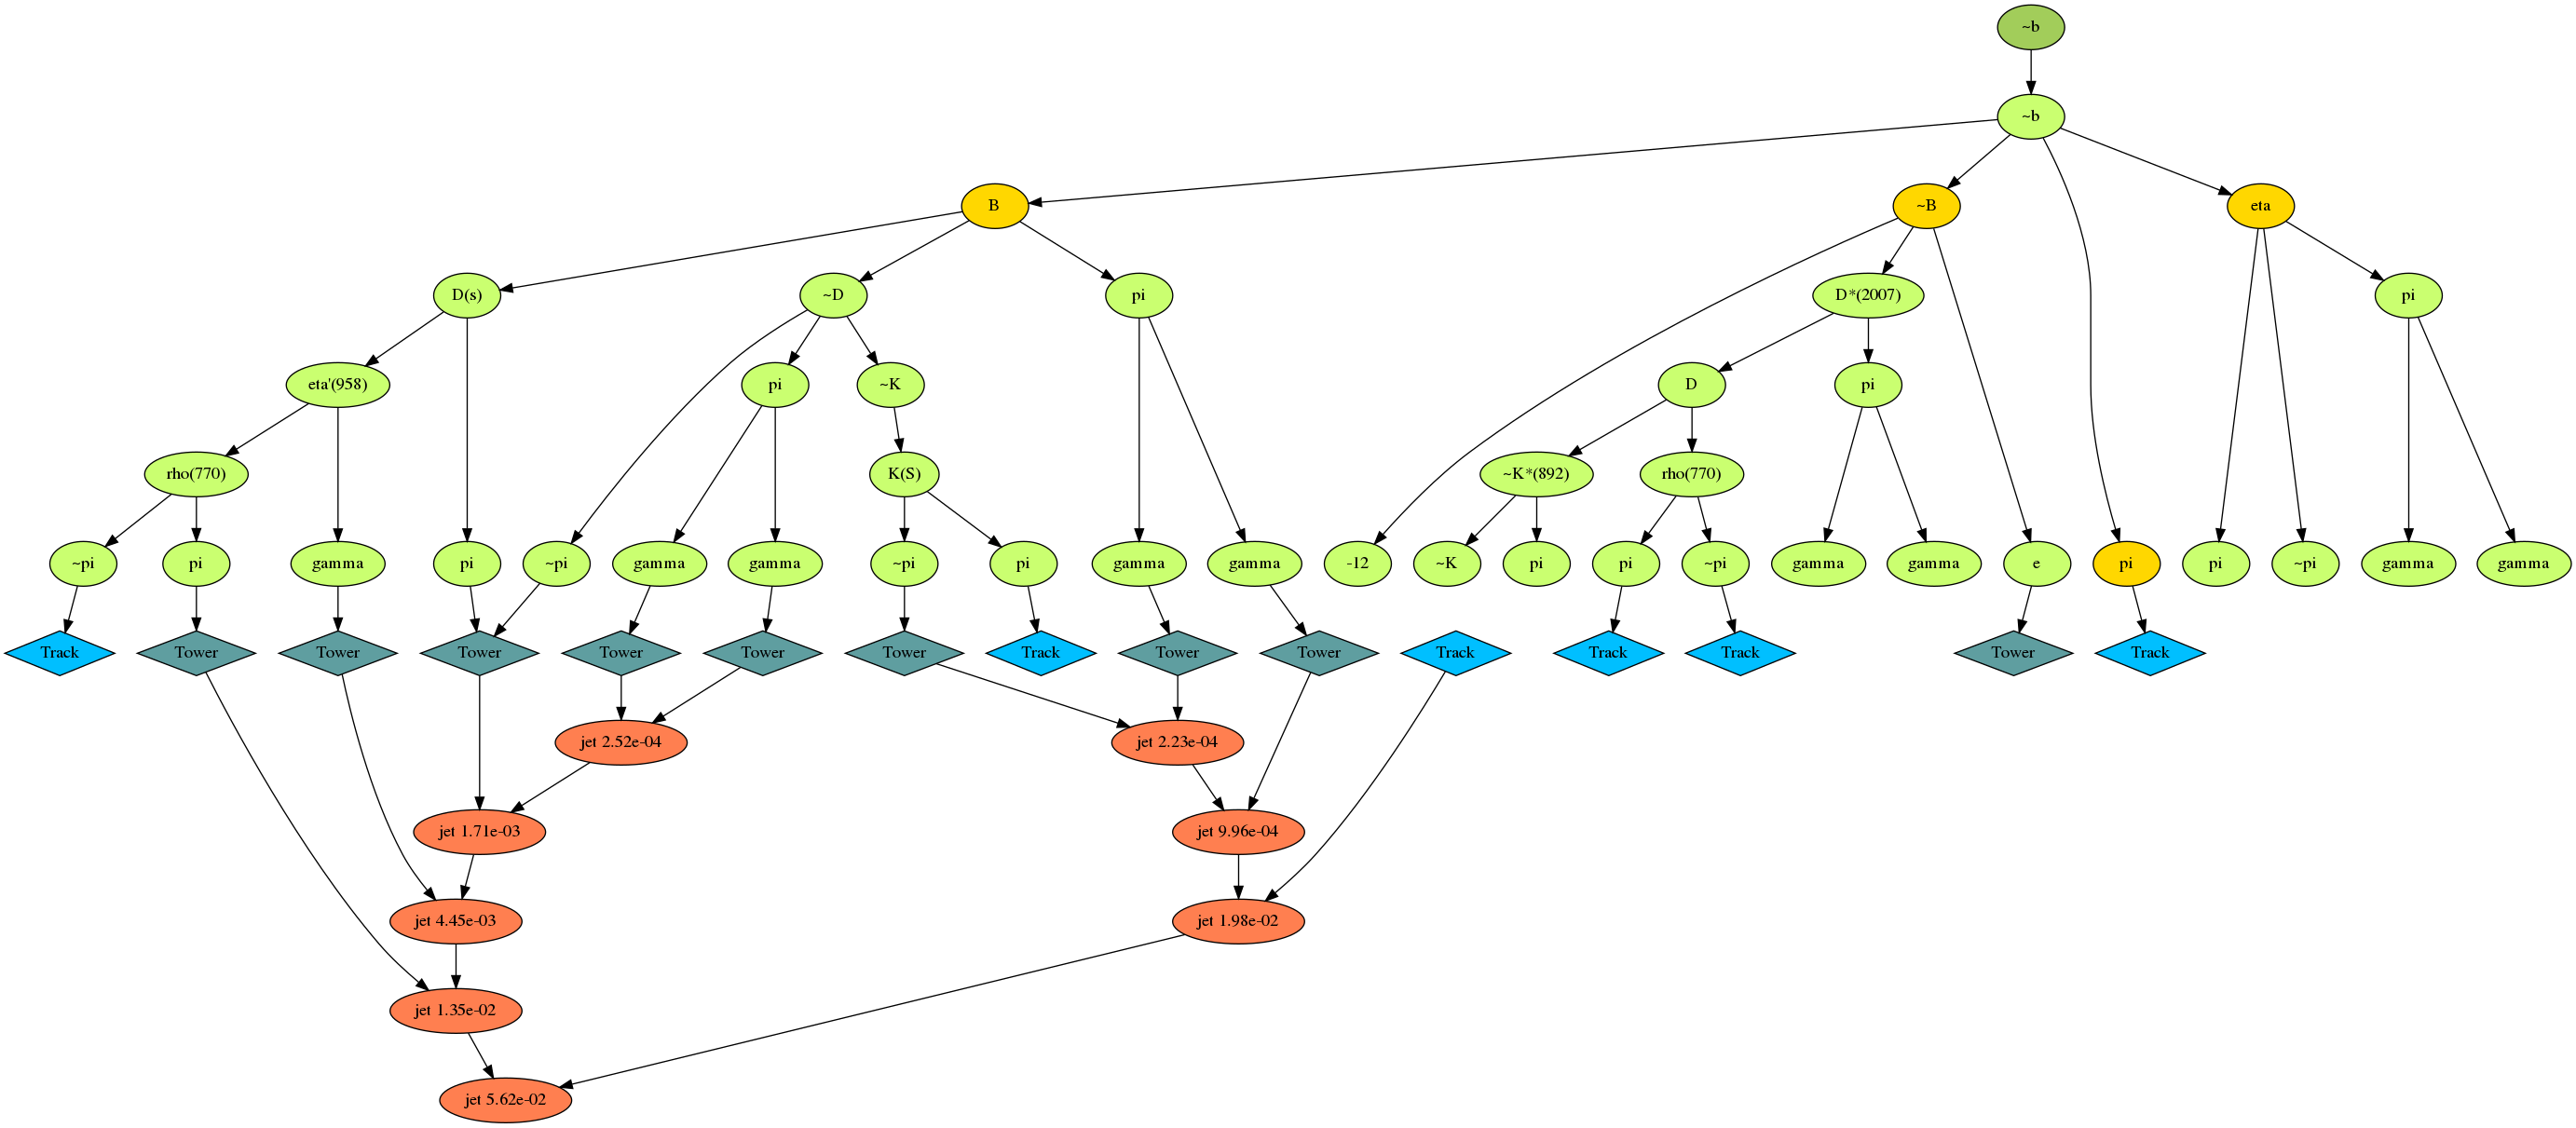
\includegraphics[width=1.\textwidth]{images/prog_bjetShower.png}
    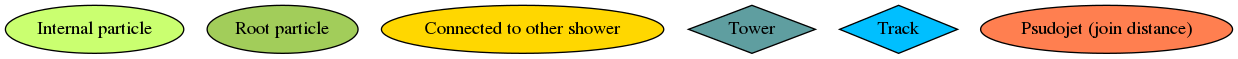
\includegraphics[width=0.5\textwidth]{images/prog_legend.png}
    \caption{A jet attempts to capture the observables let by one shower. Here we see an example shower generated in Monte Carlo.
        It was generated with aid of Madgraph~\cite{alwall_madgraph2011}, Pythia~\cite{sjostrand_pythia2015} and Delphes~\cite{deFavereau_delphesA2014}.
             The shower, and it's Monte Carlo truth is shown at the top, at the bottom
             the process of the jet clustering algorithm is seen.
         The jet clustering algorithm captures most but not all of the shower, and it captures some tracks from other parts of the event.}
    \label{fig:prog_bjetShower}
\end{sidewaysfigure}


There were a few casual observations made at this point. 
In most events, the graph of all showers is fully connected,
that is to say that the hadronisation links all showers to all other showers in most cases.
Information in one part of an event might be expected to be strongly dependant on information in the rest of the event.
This favours dealing with the event as a whole instead of jet by jet.

\begin{figure}
    \centering
    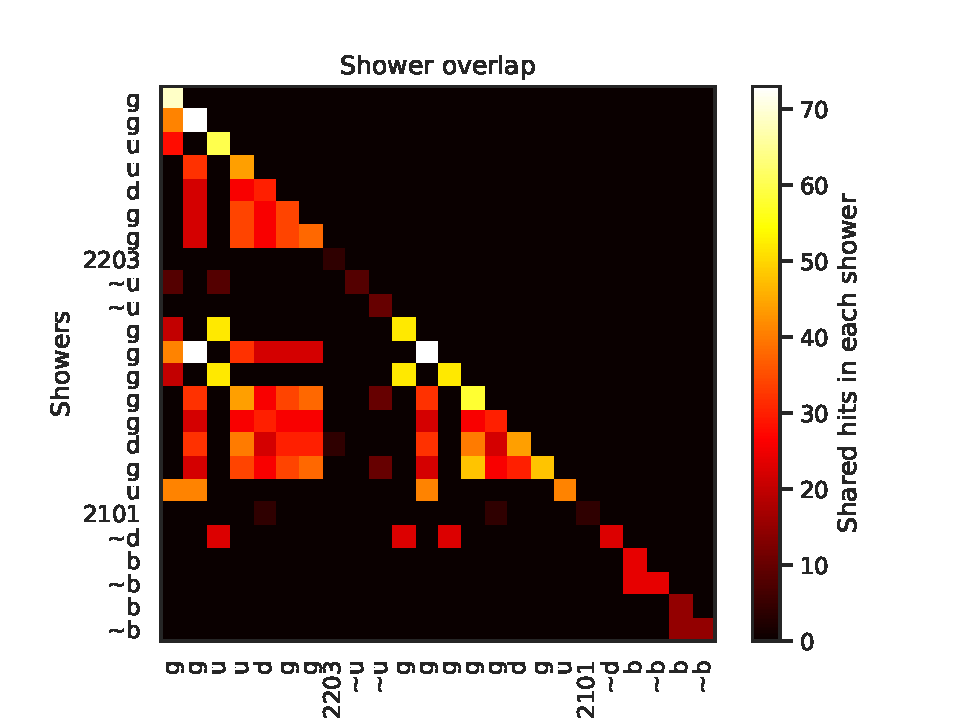
\includegraphics[width=0.8\textwidth]{images/prog_showerOverlap.pdf}
    \caption{The overlap between showers in one event. A shower is defined here as all the descendants of a particle who's parents are of the hard interaction or the proton beams.
            The axis labels identify the originating particle of the shower.
         Particles in one shower will interact with particles in another shower and then produce common descendants.
         For a shower from a colour charged this is required to form 
     colour neutral end products.}
    \label{fig:prog_showerOverlap}
\end{figure}

It also indicates that a non exclusive jet formula might make more sense - if tracks can belong to multiple showers, perhaps they should be able to belong to multiple jets.
This overlap between showers is shown for one event in figure~\ref{fig:prog_showerOverlap}.
One promising feature of this plot is that shared descendants between soft gluon showers and hard b quark showers is minimal,
so exclusive jets will merge b showers, but it looks possible to avoid excessive merging of b quark showers and soft showers.

\begin{figure}
    \centering
    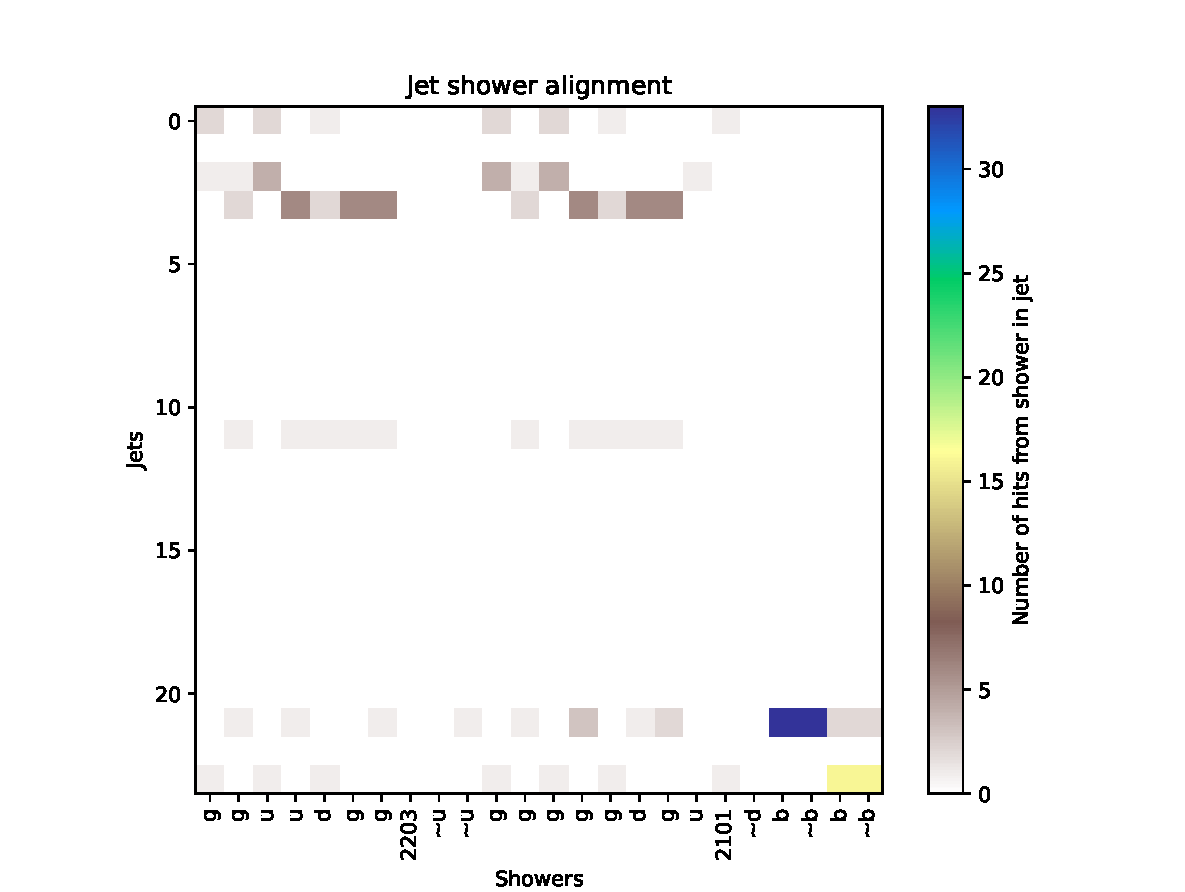
\includegraphics[width=0.8\textwidth]{images/prog_showerJetAlignment.pdf}
    \caption{The alignment between showers and jets for one event.
        The shower axis identifies the originating particle of the shower,
        the jets themselves are ordered to make the plot as close to diagonal as possible.
        Ideally each jet would capture exactly one shower
    if this occurred the plot would be diagonal.
             What is seen in this event is that many shower have be incorrectly split between many jets.}
    \label{fig:prog_showerJetAlignment}
\end{figure}

Another picture of the distinction between the signal and the soft jets can be seen in figure~\ref{fig:prog_showerJetAlignment}.
It can be seen that the hard showers fall into two jets in the bottom right of the heatmap,
and the soft showers are spread over many jets. 
This is strikingly different behaviour and one might imagine that the structure of the jet is sensitive to the nature of the shower it is built on.

It can be seen in figure~\ref{fig:prog_bjetShower} that the jet structure is not a mirror of the shower.
So the relationship between jet structure and physics is not immediately obvious, but perhaps it would be a useful structure for a classifier to combine information.
This is the inspiration for the plan to use RNTNs.


\subsection{Architectural direction}
The network used by~\cite{cheng_recursive_2018} was originally developed for parsing syntax trees.
It the case of jet clustering it generates a state vector (\(\vec{h}_k\)) for every pseudojet.
That state vector encodes the useful information about the pseudojet structure and kinematics.

The equations involved can be seen in figure~\ref{fig:plan_treeTagger}.
Qualitatively the first pseudojets being the tracks or towers must make a state vector out of the observables alone.
These are known as leaf nodes in the net, and they learn a process for encoding observables into a new hidden state.
When two pseudojets merge into a new pseudojet there are three kinds of input to the state vector;
the left and right state vectors of the child nodes and the combined kinematics of the pseudojet.
A separate procedure is learnt to combine these three things.
These two processes combine all the tracks into one root state vector.

The root state vector, or final state vector, will be passed on to a DNN,
along with global event information which tags the jet.


\begin{figure}
    \centering
    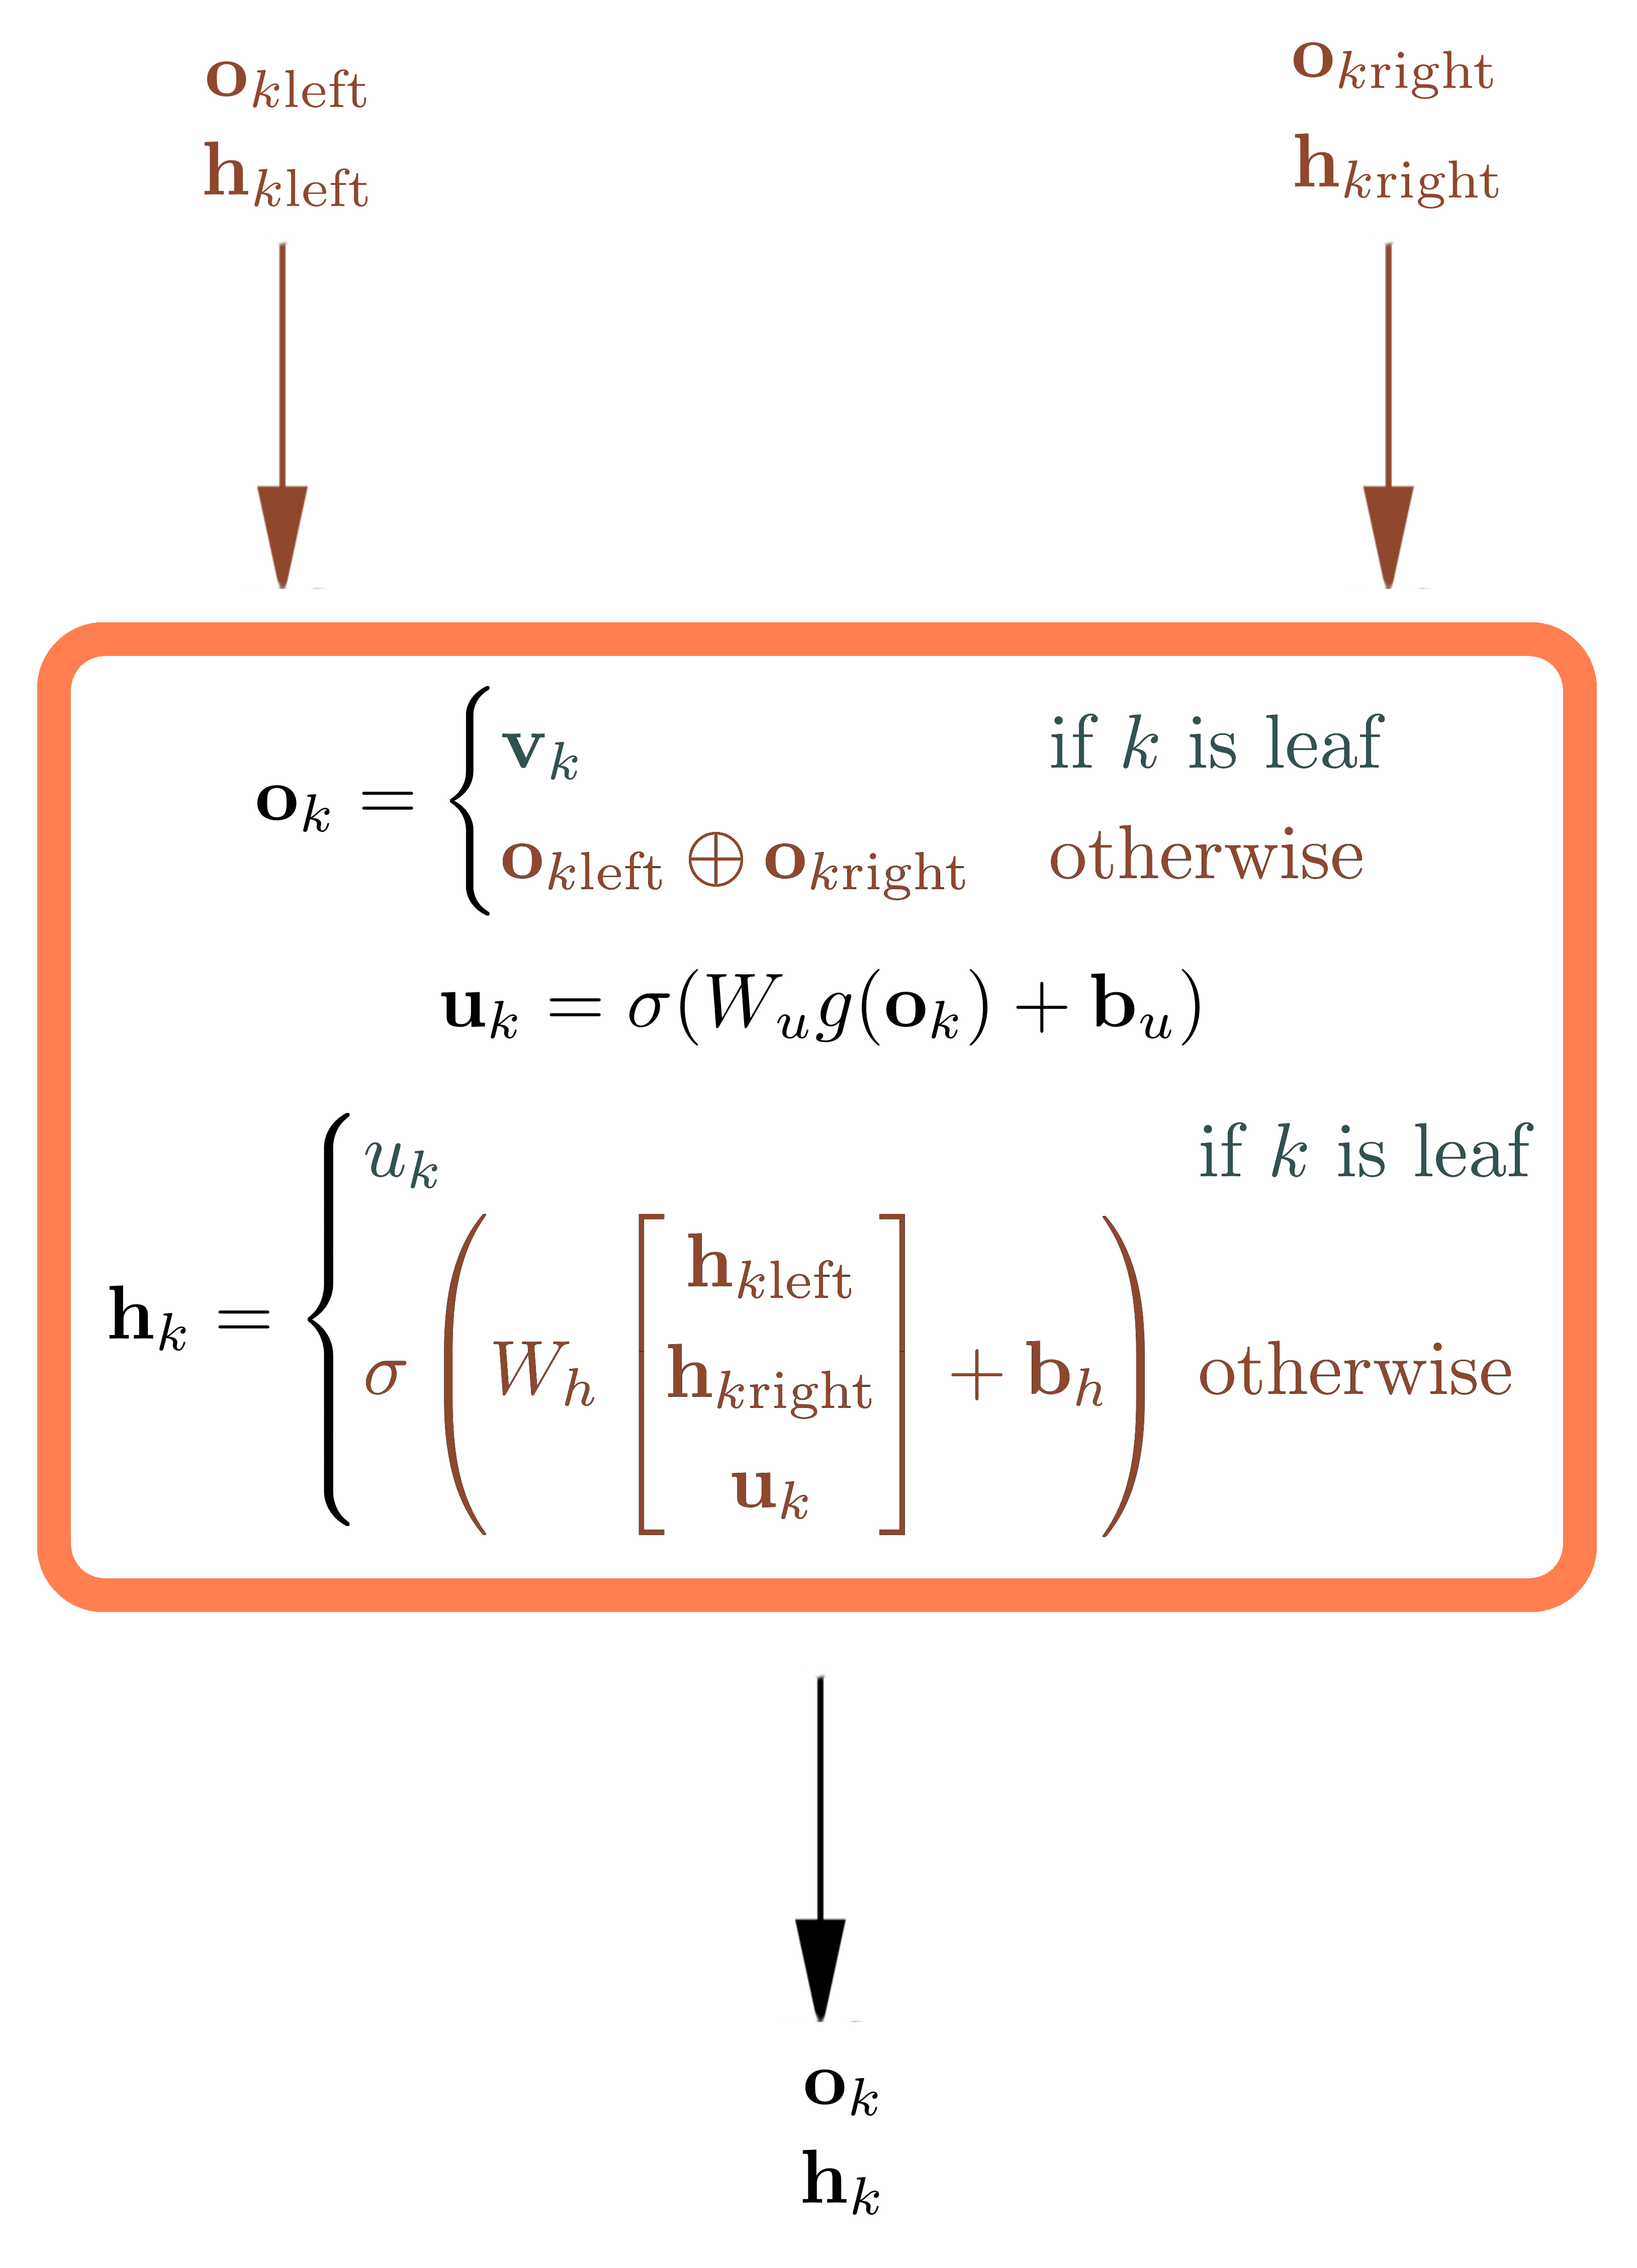
\includegraphics[width=0.5\textwidth]{images/plan_treetagger.png}
    \caption{A single node of an RNTN.
        The vector \(\vec{o}_k\) is the vector of observable properties of the \(k^\text{th}\) node. 
        If the \(k^\text{th}\) node is a leaf then these would be the track properties, otherwise they are a combination of the properties of the tracks below \(k\).
        The vector \(\vec{u}_k\) is the embedding of \(\vec{o}_k\) into the latent space of the net.
        The vector \(\vec{k}_k\) is the `state' of the \(k^\text{th}\) node, structural information about the tree propagates in the state of the nodes.
    }
    \label{fig:plan_treeTagger}
\end{figure}

\subsubsection{Subsequent steps}
Once this net has been replicated and seen to perform acceptably there are a number of forward direction open;
\begin{enumerate}
    \item Most RNNs and RNTNs have a target available at every node.
          This greatly improves the stability of the training process.
          A physically inspired intermediate target might be identified of increase the stability of the net as it trains.
    \item RNTNs have been implemented with Long Short Term Memory (LSTM) and jet taggers with LSTM have been implemented~\cite{Egan:2017ojy}.
      To my knowledge, however, they have yet to be combined.
      This would be a very natural extension.
    \item Such a net will be sensitive to the subtleties of hadronisation, 
        there would be a number of possibility's for testing their robsutness to Monte Calro errors.
        Unsupervised training on known signal/background regions in data could be compared to equivalent MC trained nets.
        Different MC generators could be compared.
    \item It would be interesting to find an interpretation of the net's latent space.
          Perhaps t-SNE would be suitable for this.
\end{enumerate}

Points 1 and 2 should certainly be undertaken, if the structure show promise then points 3 and 4 would be worth attempting.


    %\section{Acknowledgements}
    %I would like to thank Professor Stefano Moretti, Professor Claire Shepherd-Themistocleous, Professor Srinandan Dasmahapatra and Dr Emmanuel Olaiya for their excellent supervision and advice.
    %I would also like to thank Dr Mauro Verzetti for assistance with the data. 
    %The IRIDIS High Performance Computing Facility was used for this work,
    %and I am grateful for the assistance of associated support services at
    %the University of Southampton.
    \printbibliography	
\end{document}
